\documentclass[aspectratio=169, 10pt]{beamer}

% --- GÓI NGÔN NGỮ VÀ FONT CHỮ ---
\usepackage{fontspec}
\setsansfont{Arial}
\setmainfont{Arial}
\usepackage[vietnamese]{babel}

% --- TOÁN HỌC VÀ KÝ HIỆU ---
\usepackage{amsmath, amssymb, amsthm, mathtools}

% Sửa lỗi đứt đoạn dấu suy ra/tương đương do xung đột fontspec với ký hiệu ghép TeX
\renewcommand{\implies}{\ensuremath{\Rightarrow}}
\renewcommand{\Longrightarrow}{\Rightarrow}
\renewcommand{\impliedby}{\ensuremath{\Leftarrow}}
\renewcommand{\Longleftarrow}{\Leftarrow}
\renewcommand{\iff}{\ensuremath{\Leftrightarrow}}
\renewcommand{\Longleftrightarrow}{\Leftrightarrow}

% --- BẢNG BIỂU & HÌNH ẢNH ---
\usepackage{booktabs}
\usepackage{tabularx}
\usepackage{array}
\usepackage{multirow}
\usepackage{graphicx}

% --- TIKZ & ĐỒ HỌA ---
\usepackage{tikz}
\usetikzlibrary{arrows.meta, positioning, calc, shapes.geometric, backgrounds, fit}
\usepackage{tcolorbox}
\tcbuselibrary{skins}

% ==============================================================================
% CẤU HÌNH MÀU SẮC THEME XANH NƯỚC BIỂN (OCEAN BLUE PALETTE)
% ==============================================================================
\definecolor{OceanNavy}{RGB}{8, 42, 82}        % Xanh biển sâu đậm (Màu chính)
\definecolor{OceanBlue}{RGB}{20, 108, 178}     % Xanh nước biển sáng
\definecolor{OceanDeep}{RGB}{4, 28, 58}        % Xanh thẫm đại dương
\definecolor{OceanTeal}{RGB}{0, 150, 169}      % Xanh ngọc lam biển (Accent)
\definecolor{OceanCyan}{RGB}{41, 182, 246}     % Xanh lam nhạt
\definecolor{OceanLight}{RGB}{238, 246, 253}   % Nền xanh nước biển rất nhạt
\definecolor{CoralAlert}{RGB}{217, 83, 79}     % Đỏ san hô (Cảnh báo)
\definecolor{DarkText}{RGB}{33, 37, 41}        % Màu chữ chính

% Áp dụng Theme Madrid & tùy biến màu Beamer
\usetheme{Madrid}
\useinnertheme{rectangles}

% Thiết lập màu sắc hệ thống beamer
\setbeamercolor{structure}{fg=OceanBlue}
\setbeamercolor{normal text}{fg=DarkText, bg=white}
\setbeamercolor{palette primary}{fg=white, bg=OceanNavy}
\setbeamercolor{palette secondary}{fg=white, bg=OceanBlue}
\setbeamercolor{palette tertiary}{fg=white, bg=OceanDeep}
\setbeamercolor{palette quaternary}{fg=white, bg=OceanNavy}

% Tiêu đề Slide (Frametitle)
\setbeamercolor{frametitle}{fg=white, bg=OceanNavy}
\setbeamerfont{frametitle}{series=\bfseries, size=\large}

% Định dạng Block
\setbeamercolor{block title}{fg=white, bg=OceanNavy}
\setbeamercolor{block body}{fg=DarkText, bg=OceanLight}
\setbeamercolor{block title example}{fg=white, bg=OceanTeal}
\setbeamercolor{block body example}{fg=DarkText, bg=OceanLight!70!white}
\setbeamercolor{block title alerted}{fg=white, bg=CoralAlert}
\setbeamercolor{block body alerted}{fg=DarkText, bg=CoralAlert!10!white}

% Định dạng Itemize & Enumerate
\setbeamertemplate{itemize item}{\color{OceanBlue}$\blacktriangleright$}
\setbeamertemplate{itemize subitem}{\color{OceanTeal}$\bullet$}
\setbeamertemplate{itemize subsubitem}{\color{OceanCyan}\tiny$\blacksquare$}
\setbeamercolor{enumerate item}{fg=white, bg=OceanBlue}

% Thanh điều hướng dưới cùng (Footline)
\setbeamertemplate{navigation symbols}{}
\setbeamertemplate{footline}{%
  \leavevmode%
  \hbox{%
  \begin{beamercolorbox}[wd=.30\paperwidth,ht=2.4ex,dp=1.1ex,center]{palette tertiary}%
    \usebeamerfont{author in head/foot}\textbf{Nhóm K68A2} | HUS -- VNU
  \end{beamercolorbox}%
  \begin{beamercolorbox}[wd=.45\paperwidth,ht=2.4ex,dp=1.1ex,center]{palette secondary}%
    \usebeamerfont{title in head/foot}\textbf{Mô hình Lotka--Volterra Menhaden \& Bass}
  \end{beamercolorbox}%
  \begin{beamercolorbox}[wd=.25\paperwidth,ht=2.4ex,dp=1.1ex,right]{palette primary}%
    \usebeamerfont{date in head/foot}Trang \insertframenumber{} / \inserttotalframenumber\hspace*{2ex}
  \end{beamercolorbox}}%
  \vskip0pt%
}

% ==============================================================================
% THÔNG TIN TIÊU ĐỀ BÁO CÁO
% ==============================================================================
\title[\textbf{Mô hình Lotka--Volterra Menhaden \& Bass}]{\Large \textbf{ỨNG DỤNG MÔ HÌNH LOTKA--VOLTERRA MỞ RỘNG CHO HỆ SINH THÁI ATLANTIC MENHADEN -- STRIPED BASS}}
\subtitle{\normalsize Báo cáo môn học: Các mô hình toán ứng dụng}
\author[\textbf{Nhóm K68A2}]{%
  \textbf{Sinh viên thực hiện:}\\
  Tạ Tiến Nam \quad--\quad Tạ Văn Nghĩa \quad--\quad Trần Đức Kiên\\[0.12cm]
  {\small \textbf{Lớp:} K68A2 \quad|\quad \textbf{Khoa:} Toán -- Cơ -- Tin học}\\[0.12cm]
  {\small \textbf{Giảng viên hướng dẫn:} TS. Nguyễn Trọng Hiếu}
}
\institute[\textbf{HUS -- VNU}]{%
  \textbf{ĐẠI HỌC QUỐC GIA HÀ NỘI -- TRƯỜNG ĐẠI HỌC KHOA HỌC TỰ NHIÊN}
}
\date{Hà Nội, 2026}

% ==============================================================================
% BẮT ĐẦU NỘI DUNG SLIDE
% ==============================================================================
\begin{document}

% ------------------------------------------------------------------------------
% SLIDE 1: TRANG TIÊU ĐỀ (TITLE SLIDE)
% ------------------------------------------------------------------------------
\begin{frame}[plain]
  \begin{tikzpicture}[remember picture, overlay]
    % Banner nền trên cùng (Ocean Blue gradient)
    \fill[OceanNavy] (current page.north west) rectangle ($(current page.north east) + (0, -2.4cm)$);
    \fill[OceanTeal] ($(current page.north west) + (0, -2.4cm)$) rectangle ($(current page.north east) + (0, -2.55cm)$);
    
    % Dải chân trang
    \fill[OceanNavy] (current page.south west) rectangle ($(current page.south east) + (0, 0.7cm)$);
    \node[white, font=\footnotesize, above=0.15cm] at (current page.south) {TRƯỜNG ĐẠI HỌC KHOA HỌC TỰ NHIÊN -- ĐẠI HỌC QUỐC GIA HÀ NỘI};
  \end{tikzpicture}

  \vspace*{-0.4cm}
  \begin{columns}[c]
    \begin{column}{0.18\textwidth}
      \centering
      \IfFileExists{logo_hus.png}{%
        
\includegraphics[height=1.8cm, keepaspectratio]{logo_hus.png}
      }{%
        \begin{tikzpicture}
          \draw[thick, white, fill=OceanBlue!60] (0,0) circle (0.9cm);
          \node[white, font=\scriptsize\bfseries, align=center] at (0,0) {HUS\\VNU};
        \end{tikzpicture}
      }
    \end{column}
    \begin{column}{0.80\textwidth}
      {\color{white}\small \textbf{KHOA TOÁN -- CƠ -- TIN HỌC $\bullet$ BỘ MÔN TOÁN ỨNG DỤNG}}\\[2pt]
      {\color{white}\large \textbf{BÁO CÁO TIỂU LUẬN: CÁC MÔ HÌNH TOÁN ỨNG DỤNG}}
    \end{column}
  \end{columns}

  \vspace{0.6cm}

  \begin{center}
    \begin{tcolorbox}[colback=OceanLight, colframe=OceanBlue, arc=2mm, width=0.98\textwidth, boxrule=1.2pt]
      \centering
      {\color{OceanNavy}\large \textbf{ỨNG DỤNG MÔ HÌNH LOTKA--VOLTERRA MỞ RỘNG}}\\[3pt]
      {\color{OceanNavy}\large \textbf{CHO HỆ SINH THÁI ATLANTIC MENHADEN -- STRIPED BASS}}\\[4pt]
      {\color{OceanTeal}\footnotesize \textit{Phân tích động thái 2 loài, dữ liệu thực tế Vịnh Chesapeake và Khuyến nghị chính sách khai thác}}
    \end{tcolorbox}
  \end{center}

  \vspace{0.1cm}

  \begin{columns}[t]
    \begin{column}{0.50\textwidth}
      \begin{tcolorbox}[colback=white, colframe=OceanNavy!40, arc=1.5mm, boxrule=0.8pt, title={\color{OceanNavy}\footnotesize\textbf{Sinh viên thực hiện (K68A2)}}]
        \footnotesize
        $\bullet$ \textbf{Tạ Tiến Nam} -- MSV: 23000143\\
        $\bullet$ \textbf{Tạ Văn Nghĩa} -- MSV: 23000145\\
        $\bullet$ \textbf{Trần Đức Kiên} -- MSV: 23000131
      \end{tcolorbox}
    \end{column}
    \begin{column}{0.48\textwidth}
      \begin{tcolorbox}[colback=white, colframe=OceanTeal!60, arc=1.5mm, boxrule=0.8pt, title={\color{OceanTeal}\footnotesize\textbf{Cán bộ hướng dẫn}}]
        \footnotesize
        $\bullet$ \textbf{TS. Nguyễn Trọng Hiếu}\\[2pt]
        \textit{Khoa Toán -- Cơ -- Tin học}\\
        \textit{ĐH Khoa học Tự nhiên, ĐHQGHN}
      \end{tcolorbox}
    \end{column}
  \end{columns}
\end{frame}


% ==============================================================================
% SLIDE 2: MỤC LỤC NỘI DUNG BÁO CÁO (AGENDA)
% ------------------------------------------------------------------------------
\begin{frame}{Mục lục nội dung báo cáo}
  \vspace*{-0.15cm}
  \begin{columns}[t]
    \begin{column}{0.48\textwidth}
      \begin{tcolorbox}[colback=OceanLight, colframe=OceanNavy, arc=1.5mm, boxrule=0.7pt, top=1.0mm, bottom=1.0mm, left=2mm, right=2mm, title={\textbf{1. Bối cảnh nghiên cứu \& Đặt vấn đề}}]
        \scriptsize
        $\blacktriangleright$ Hệ sinh thái Vịnh Chesapeake \& 2 loài cá\\
        $\blacktriangleright$ Khủng hoảng khai thác \& Chuyển dịch EBFM
      \end{tcolorbox}
      
      \vspace{0.12cm}
      
      \begin{tcolorbox}[colback=OceanLight, colframe=OceanBlue, arc=1.5mm, boxrule=0.7pt, top=1.0mm, bottom=1.0mm, left=2mm, right=2mm, title={\textbf{2. Mô hình sinh thái \& Khớp tham số}}]
        \scriptsize
        $\blacktriangleright$ Hệ Lotka--Volterra mở rộng \& Khớp NLS 23 năm\\
        $\blacktriangleright$ Điểm dừng tự nhiên $Q$ \& Độ đàn hồi sinh thái
      \end{tcolorbox}

      \vspace{0.12cm}
      
      \begin{tcolorbox}[colback=OceanLight, colframe=OceanTeal, arc=1.5mm, boxrule=0.7pt, top=1.0mm, bottom=1.0mm, left=2mm, right=2mm, title={\textbf{3. Mô hình sinh học--kinh tế (Chương 3)}}]
        \scriptsize
        $\blacktriangleright$ Hàm CPUE, lợi nhuận $\pi$ \& Bị chặn trong $\Omega$\\
        $\blacktriangleright$ 4 điểm cân bằng bionomic \& Thời gian hồi phục $\tau$
      \end{tcolorbox}
    \end{column}

    \begin{column}{0.48\textwidth}
      \begin{tcolorbox}[colback=OceanLight, colframe=OceanNavy!75!OceanBlue, arc=1.5mm, boxrule=0.7pt, top=1.0mm, bottom=1.0mm, left=2mm, right=2mm, title={\textbf{4. Chính sách khai thác nghề cá}}]
        \scriptsize
        $\blacktriangleright$ Đánh giá 3 chính sách: MSY, MEY và RMY\\
        $\blacktriangleright$ Động lực chuyển tiếp \& Nguy cơ đổ vỡ sinh thái
      \end{tcolorbox}
      
      \vspace{0.12cm}

      \begin{tcolorbox}[colback=OceanLight, colframe=OceanTeal!80!OceanNavy, arc=1.5mm, boxrule=0.7pt, top=1.0mm, bottom=1.0mm, left=2mm, right=2mm, title={\textbf{5. Phân tích độ nhạy cục bộ (DDM)}}]
        \scriptsize
        $\blacktriangleright$ Phương pháp đạo hàm trực tiếp DDM theo 6 tham số\\
        $\blacktriangleright$ Bất đối xứng nhạy cảm giữa loài mồi và thú ăn thịt
      \end{tcolorbox}

      \vspace{0.12cm}

      \begin{tcolorbox}[colback=OceanLight, colframe=CoralAlert!90!OceanNavy, arc=1.5mm, boxrule=0.7pt, top=1.0mm, bottom=1.0mm, left=2mm, right=2mm, title={\textbf{6. Tổng kết \& Khuyến nghị quản lý}}]
        \scriptsize
        $\blacktriangleright$ Bác bỏ MSY đơn loài $\implies$ Khuyến nghị EBFM\\
        $\blacktriangleright$ 4 giải pháp quản lý nghề cá bền vững tại Vịnh
      \end{tcolorbox}
    \end{column}
  \end{columns}
\end{frame}

% ==============================================================================
% PHẦN 1: BỐI CẢNH NGHIÊN CỨU & ĐẶT VẤN ĐỀ (CHƯƠNG 1)
% ==============================================================================
\section{Bối cảnh nghiên cứu \& Đặt vấn đề}

% ------------------------------------------------------------------------------
% SLIDE 3: BỐI CẢNH VỊNH CHESAPEAKE
% ------------------------------------------------------------------------------
\begin{frame}{Bối cảnh nghiên cứu: Hệ sinh thái Vịnh Chesapeake}
  \begin{columns}[c]
    \begin{column}{0.54\textwidth}
      \begin{block}{\textbf{Vịnh Chesapeake -- Cửa sông lớn nhất Bắc Mỹ}}
        \footnotesize
        \begin{itemize}
          \item Nằm ở bờ Đông nước Mỹ (tiếp giáp Virginia, Maryland).
          \item Môi trường sống thiết yếu cho hơn \textbf{3.600 loài} sinh vật; ngư trường sinh kế cho hàng triệu người dân duyên hải.
          \item Độ nhạy cảm sinh thái cực cao trước ô nhiễm, bão lũ và đánh bắt nhân tạo.
        \end{itemize}
      \end{block}

      \vspace{0.1cm}

      \begin{block}{\textbf{Mâu thuẫn then chốt}}
        \footnotesize
        \begin{itemize}
          \item \textbf{Kinh tế:} Nhu cầu tối đa hóa sản lượng đánh bắt ngắn hạn.
          \item \textbf{Sinh thái:} Nguy cơ đổ vỡ chuỗi thức ăn (\textit{trophic cascade}) và suy thoái nguồn tài nguyên sinh khối vĩnh viễn.
        \end{itemize}
      \end{block}
    \end{column}

    \begin{column}{0.44\textwidth}
      \begin{tcolorbox}[colback=OceanLight, colframe=OceanNavy, arc=2mm, title={\centering \textbf{Cặp loài tương tác trọng yếu}}]
        \footnotesize
        Nghiên cứu của \textbf{Panayotova et al. (2023)} trên tạp chí \textit{Ecological Modelling} tập trung vào:
        \vspace{0.15cm}
        
        \begin{center}
          \begin{tikzpicture}
            \node[draw=OceanNavy, fill=white, rounded corners=2mm, text width=4.3cm, align=center, thick] (prey) {
              \textbf{Cá mòi dầu Đại Tây Dương}\\
              (\textit{Brevoortia tyrannus})\\
              \scriptsize $\blacktriangleright$ Con mồi (\textit{Prey}) $x(t)$
            };
            \node[draw=OceanNavy, fill=white, rounded corners=2mm, text width=4.3cm, align=center, thick, below=0.45cm of prey] (pred) {
              \textbf{Cá vược sọc (Rockfish)}\\
              (\textit{Morone saxatilis})\\
              \scriptsize $\blacktriangleright$ Săn mồi (\textit{Predator}) $y(t)$
            };
            \draw[<->, >=stealth, line width=1.3pt, color=CoralAlert] (prey) -- node[right, font=\tiny, align=left] {Lưới\\thức ăn} (pred);
          \end{tikzpicture}
        \end{center}
      \end{tcolorbox}
    \end{column}
  \end{columns}
\end{frame}

% ------------------------------------------------------------------------------
% SLIDE 4A: CÁ MÒI DẦU (MENHADEN)
% ------------------------------------------------------------------------------
\begin{frame}{Hai loài sinh vật trọng yếu: Cá mòi dầu (\textit{Brevoortia tyrannus})}
  \begin{columns}[c]
    \begin{column}{0.44\textwidth}
      \begin{tcolorbox}[colback=white, colframe=OceanNavy!30, arc=2mm, boxrule=0.8pt, width=\linewidth, halign=center, top=1.5mm, bottom=1.5mm]
        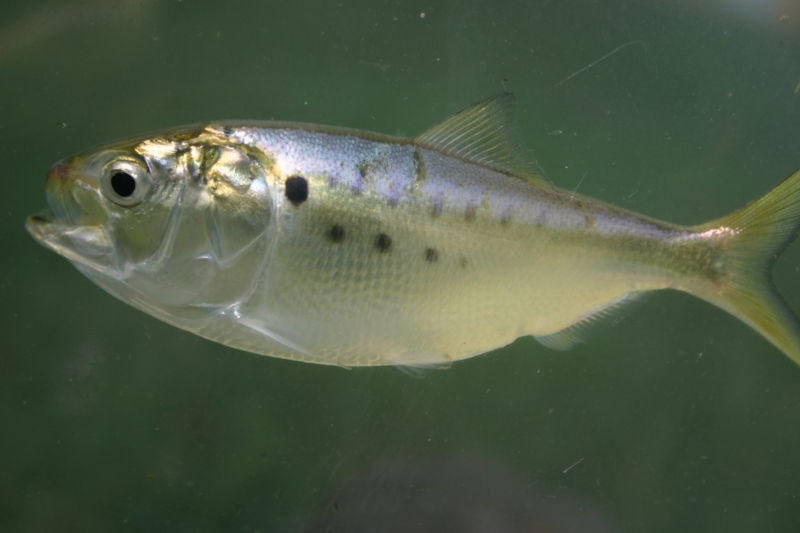
\includegraphics[width=\linewidth, height=3.6cm, keepaspectratio]{images/ca_moi_dau.jpg}\\[4pt]
        {\footnotesize \textbf{Cá mòi dầu Đại Tây Dương} (\textit{Menhaden})}
      \end{tcolorbox}

      \vspace{0.1cm}
      
      \begin{tcolorbox}[colback=OceanLight, colframe=OceanNavy, arc=1.5mm, top=1.2mm, bottom=1.2mm]
        \scriptsize
        $\blacktriangleright$ \textbf{Vai trò mô hình:} Quần thể con mồi $x(t)$\\
        $\blacktriangleright$ \textbf{Biệt danh:} \textit{``Loài cá quan trọng nhất đại dương''}
      \end{tcolorbox}
    \end{column}

    \begin{column}{0.54\textwidth}
      \begin{block}{\textbf{Đặc điểm sinh học \& Vai trò sinh thái}}
        \footnotesize
        \begin{itemize}
          \setlength{\itemsep}{3pt}
          \item \textbf{Sinh học:} Dài $\sim 45\text{ cm}$, bơi thành đàn khổng lồ tại tầng mặt ven bờ; sinh sản quanh năm.
          \item \textbf{Ăn lọc (\textit{Filter-feeder}):} Tiêu thụ tảo phù du, \textbf{chống phú dưỡng hóa}, giữ sạch nước vịnh.
          \item \textbf{Nền tảng chuỗi thức ăn:} Thức ăn của cá vược sọc, cá xanh, cá mập cát, chim ưng biển (\textit{Osprey}).
          \item \textbf{Kinh tế:} Làm bột cá, mồi câu cua xanh, ép dầu giàu axit béo \textbf{Omega-3} (EPA/DHA) giá trị cao.
        \end{itemize}
      \end{block}
    \end{column}
  \end{columns}
\end{frame}

% ------------------------------------------------------------------------------
% SLIDE 4B: CÁ VƯỢC SỌC (STRIPED BASS)
% ------------------------------------------------------------------------------
\begin{frame}{Hai loài sinh vật trọng yếu: Cá vược sọc (\textit{Morone saxatilis})}
  \begin{columns}[c]
    \begin{column}{0.44\textwidth}
      \begin{tcolorbox}[colback=white, colframe=OceanTeal!40, arc=2mm, boxrule=0.8pt, width=\linewidth, halign=center, top=1.5mm, bottom=1.5mm]
        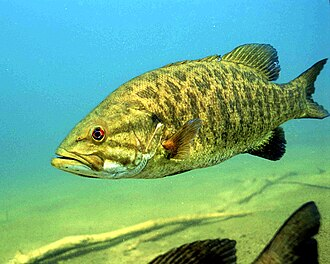
\includegraphics[width=\linewidth, height=3.6cm, keepaspectratio]{images/ca_vuoc_soc.jpg}\\[4pt]
        {\footnotesize \textbf{Cá vược sọc} (\textit{Striped Bass / Rockfish})}
      \end{tcolorbox}

      \vspace{0.1cm}

      \begin{tcolorbox}[colback=OceanLight, colframe=OceanTeal, arc=1.5mm, top=1.2mm, bottom=1.2mm]
        \scriptsize
        $\blacktriangleright$ \textbf{Vai trò mô hình:} Quần thể kẻ săn mồi $y(t)$\\
        $\blacktriangleright$ \textbf{Biểu tượng:} \textit{Kẻ săn mồi đỉnh cao \& Chỉ thị sức khỏe vịnh}
      \end{tcolorbox}
    \end{column}

    \begin{column}{0.54\textwidth}
      \begin{exampleblock}{\textbf{Đặc điểm sinh học \& Tầm quan trọng nghề cá}}
        \footnotesize
        \begin{itemize}
          \setlength{\itemsep}{3pt}
          \item \textbf{Sinh học:} Kích thước lớn ($60 - 90\text{ cm}$, $5 - 15\text{ kg}$), di cư ngược dòng (\textit{anadromous}) vào sông đẻ trứng.
          \item \textbf{Tập tính săn mồi:} Cá mòi dầu chiếm tỷ trọng áp đảo trong khẩu phần sinh khối và năng lượng trao đổi chất.
          \item \textbf{Nghề cá thương mại:} Cung cấp thịt cá thương phẩm cao cấp cho chuỗi nhà hàng trên toàn quốc.
          \item \textbf{Nghề cá giải trí:} Ngành câu cá thu hút hàng trăm nghìn cần thủ, đóng góp \textbf{hàng tỷ USD vào GDP}.
        \end{itemize}
      \end{exampleblock}
    \end{column}
  \end{columns}
\end{frame}

% ------------------------------------------------------------------------------
% SLIDE 5: KHỦNG HOẢNG KHAI THÁC & BI KỊCH TÀI NGUYÊN CHUNG
% ------------------------------------------------------------------------------
\begin{frame}{Khủng hoảng khai thác \& Bi kịch tài nguyên chung}
  \begin{columns}[t]
    \begin{column}{0.50\textwidth}
      \begin{alertblock}{\textbf{Thực trạng suy giảm nghiêm trọng}}
        \footnotesize
        \begin{itemize}
          \item \textbf{Cá mòi dầu:} Sinh khối giảm sút liên tục từ thập niên 1970 do tàu công nghiệp dùng lưới vây khổng lồ (\textit{purse seine}) phối hợp máy bay trinh sát càn quét.
          \item \textbf{Cá vược sọc:} Bị xếp vào diện \textbf{đang bị đánh bắt quá mức} (\textit{overfished}) theo Báo cáo NEFSC (2019).
          \item \textbf{Hệ lụy kép:} Thiếu cá mòi dầu khiến cá vược sọc suy dinh dưỡng, suy giảm miễn dịch và bùng phát dịch bệnh lao cá do \textit{Mycobacteriosis}.
        \end{itemize}
      \end{alertblock}
    \end{column}

    \begin{column}{0.48\textwidth}
      \begin{block}{\textbf{Bi kịch tài nguyên chung (\textit{Hardin, 1968})}}
        \footnotesize
        \begin{itemize}
          \item Ngư trường là tài sản sở hữu chung mở.
          \item Từng tàu cá chạy đua tối đa hóa sản lượng trước mắt, bỏ qua ngoại ứng tiêu cực (\textit{negative externalities}) làm cạn kiệt khả năng tái sinh của nguồn tài nguyên.
        \end{itemize}
      \end{block}

      \vspace{0.1cm}

      \begin{exampleblock}{\textbf{Nghịch lý đánh giá trữ lượng đơn loài}}
        \footnotesize
        Báo cáo SEDAR 69 (2020) cho rằng cá mòi dầu ``chưa bị đánh bắt quá mức'' vì chỉ tính theo mô hình đơn loài! Bỏ qua hoàn toàn nhu cầu thức ăn sống còn của cá vược sọc!
      \end{exampleblock}
    \end{column}
  \end{columns}
\end{frame}

% ------------------------------------------------------------------------------
% SLIDE 6: CHUYỂN DỊCH SANG QUẢN LÝ DỰA TRÊN HỆ SINH THÁI (EBFM)
% ------------------------------------------------------------------------------
\begin{frame}{Nhu cầu chuyển dịch sang Quản lý Dựa trên Hệ sinh thái (EBFM)}
  \begin{columns}[c]
    \begin{column}{0.50\textwidth}
      \begin{tcolorbox}[colback=red!5!white, colframe=CoralAlert, arc=2mm, title=\textbf{Quản lý đơn loài truyền thống}]
        \footnotesize
        \begin{itemize}
          \item Xem xét từng quần thể cá độc lập.
          \item Giả định tốc độ sinh khối chỉ phụ thuộc vào số lượng nội bộ loài và nỗ lực đánh bắt.
          \item \textbf{Hậu quả nguy hại:} Đánh bắt tối đa cá mòi dầu sẽ làm sụp đổ nguồn thức ăn, đẩy đàn cá vược sọc vào nguy cơ tuyệt chủng.
        \end{itemize}
      \end{tcolorbox}
    \end{column}

    \begin{column}{0.50\textwidth}
      \begin{tcolorbox}[colback=OceanLight, colframe=OceanNavy, arc=2mm, title=\textbf{Quản lý dựa trên hệ sinh thái (EBFM)}]
        \footnotesize
        \begin{itemize}
          \item Xem xét toàn diện tương tác trong mạng lưới thức ăn.
          \item Thiết lập \textbf{Điểm tham chiếu sinh thái} (\textit{ERP}).
          \item Nghiên cứu của Howell et al. (2021) khuyến nghị: Hạn ngạch cá mồi cần phải \textbf{cắt giảm ít nhất 40\% -- 50\%} so với mô hình đơn loài để bảo tồn loài săn mồi!
        \end{itemize}
      \end{tcolorbox}
    \end{column}
  \end{columns}

  
\end{frame}



% ==============================================================================
% PHẦN 2: MÔ HÌNH TOÁN HỌC LOTKA--VOLTERRA TỔNG QUÁT (CHƯƠNG 2)
% ==============================================================================
\section{Mô hình Lotka--Volterra mở rộng}

% ------------------------------------------------------------------------------
% SLIDE 8: HỆ PHƯƠNG TRÌNH & Ý NGHĨA THAM SỐ LOTKA--VOLTERRA MỞ RỘNG
% ------------------------------------------------------------------------------
\begin{frame}{Hệ phương trình vi phân Lotka--Volterra \& Ý nghĩa tham số}
  \vspace*{-0.2cm}
  \begin{block}{\textbf{Mô hình Lotka--Volterra mở rộng 2 loài (Panayotova et al., 2023)}}
    \footnotesize
    Tốc độ biến thiên sinh khối con mồi $x(t)$ (cá mòi dầu) và kẻ săn mồi $y(t)$ (cá vược sọc):
    \begin{equation}
    \label{eq:lv_system}
    \left\{
    \begin{aligned}
    \frac{dx}{dt} &= x(\mathbf{r} - \mathbf{a}x - \mathbf{b}y) \\
    \frac{dy}{dt} &= y(-\mathbf{e} - \mathbf{c}y + \mathbf{d}x)
    \end{aligned}
    \right.
    \end{equation}
  \end{block}

  \vspace{0.05cm}

  \begin{center}
  \scriptsize
  \renewcommand{\arraystretch}{1.10}
  \begin{tabularx}{\textwidth}{c l X}
    \toprule
    \textbf{Tham số} & \textbf{Ý nghĩa sinh học} & \textbf{Vai trò trong hệ sinh thái} \\
    \midrule
    \multicolumn{3}{l}{\textbf{\color{OceanNavy}$\blacktriangleright$ Tham số thuộc phương trình con mồi $x(t)$ (Cá mòi dầu):}} \\
    $r > 0$ & Tốc độ tăng trưởng nội tại & Khả năng sinh sản tối đa của cá mòi dầu khi mật độ thấp \\
    $a > 0$ & Hệ số tự giới hạn logistic & Cạnh tranh nội bộ về thức ăn (tảo phù du) và không gian ven bờ \\
    $b > 0$ & Hệ số săn bắt của cá vược sọc & Tỷ lệ cá mòi dầu bị tiêu thụ trên mỗi đơn vị gặp gỡ giữa 2 loài \\
    \midrule
    \multicolumn{3}{l}{\textbf{\color{OceanNavy}$\blacktriangleright$ Tham số thuộc phương trình kẻ săn mồi $y(t)$ (Cá vược sọc):}} \\
    $e > 0$ & Tỷ lệ tử vong tự nhiên & Mức chết tự nhiên của cá vược sọc khi hoàn toàn thiếu thức ăn \\
    $c > 0$ & Hệ số tự giới hạn mật độ & Cạnh tranh bãi đẻ nước ngọt và mật độ quần thể nội bộ loài \\
    $d > 0$ & Hiệu quả chuyển hóa sinh khối & Năng lượng tiêu thụ cá mòi dầu chuyển hóa thành cá thể mới \\
    \bottomrule
  \end{tabularx}
  \end{center}
\end{frame}

% ------------------------------------------------------------------------------
% SLIDE 10: GIẢ THIẾT NỀN TẢNG & ƯU THẾ MÔ HÌNH
% ------------------------------------------------------------------------------
\begin{frame}{5 Giả thiết nền tảng \& Ưu thế của mô hình}
  \begin{columns}[t]
    \begin{column}{0.50\textwidth}
      \begin{block}{\textbf{5 Giả thiết sinh học nền tảng}}
        \footnotesize
        \begin{enumerate}
          \item \textbf{Tăng trưởng logistic của con mồi:} Khi $y=0$, $\dot{x} = rx(1 - x/K_x)$ với $K_x = r/a$.
          \item \textbf{Thức ăn duy nhất:} Cá mòi dầu là nguồn thức ăn chính duy trì đàn cá vược sọc.
          \item \textbf{Suy giảm hàm mũ:} Khi $x=0$, đàn săn mồi suy tàn nhanh về 0.
          \item \textbf{Hệ sinh thái cô lập:} Bỏ qua tương tác với loài thứ yếu và biến động ngẫu nhiên khí hậu.
          \item \textbf{Đồng nhất cấu trúc:} Không phân biệt tuổi, kích thước cá thể và phân bố địa lý.
        \end{enumerate}
      \end{block}
    \end{column}

    \begin{column}{0.48\textwidth}
      \begin{exampleblock}{\textbf{Ưu thế vượt trội của mô hình}}
        \footnotesize
        \begin{itemize}
          \item \textit{Analytically tractable}: Số lượng tham số vừa đủ để giải tích tường minh các điểm cân bằng, Jacobi và tính ổn định.
          \item \textit{Phase-shift}: Mô tả chính xác quy luật dao động bùng nổ -- suy giảm tự nhiên giữa 2 loài.
          \item \textit{Overfitting}: Quy mô 6 tham số là tối ưu để khớp tin cậy với chuỗi dữ liệu 23 năm thực tế.
        \end{itemize}
      \end{exampleblock}
    \end{column}
  \end{columns}
\end{frame}

% ==============================================================================
% PHẦN 3: DỮ LIỆU THỰC TẾ & KHỚP THAM SỐ (CHƯƠNG 2)
% ==============================================================================
\section{Dữ liệu thực tế \& Khớp tham số}

% ------------------------------------------------------------------------------
% SLIDE 11: NGUỒN DỮ LIỆU THỰC NGHIỆM & BỘ THAM SỐ TỐI ƯU
% ------------------------------------------------------------------------------
\begin{frame}{Nguồn dữ liệu thực nghiệm \& Bộ tham số tối ưu}
  \begin{columns}[c]
    \begin{column}{0.46\textwidth}
      \begin{block}{\textbf{Nguồn dữ liệu thực tế (ASMFC)}}
        \footnotesize
        \begin{itemize}
          \setlength{\itemsep}{3pt}
          \item Chuỗi số liệu độ phong phú cá thể (\textit{abundance}) trong \textbf{23 năm (1995 -- 2017)}.
          \item \textbf{Cá mòi dầu:} SEDAR 69 -- Benchmark Stock Assessment (2019).
          \item \textbf{Cá vược sọc:} 2022 ASMFC Stock Assessment Update Report.
          \item Chuẩn hóa chia cho $10^9$ (\textbf{tỷ con}) để tối ưu tính toán số học.
        \end{itemize}
      \end{block}

      \vspace{0.15cm}

      \begin{tcolorbox}[colback=OceanLight, colframe=OceanNavy, arc=1.5mm, top=1.2mm, bottom=1.2mm]
        \scriptsize
        $\blacktriangleright$ \textbf{Phương pháp ước lượng:} Hồi quy phi tuyến bình phương tối thiểu (NLS).\\
        $\blacktriangleright$ \textbf{Độ chính xác:} Sai số chuẩn phần dư $S = \mathbf{0.11}$ tỷ con (mô hình khớp xuất sắc dữ liệu thực tế).
      \end{tcolorbox}
    \end{column}

    \begin{column}{0.52\textwidth}
      \begin{block}{\textbf{Bộ tham số tối ưu từ khớp NLS}}
        \centering
        \footnotesize
        \renewcommand{\arraystretch}{1.12}
        \begin{tabular}{c l c}
          \toprule
          \textbf{Tham số} & \textbf{Ý nghĩa sinh học} & \textbf{Giá trị tối ưu} \\
          \midrule
          $r$ & Tăng trưởng cá mòi dầu & $\mathbf{0.513}\ \text{năm}^{-1}$ \\
          $a$ & Tự giới hạn cá mòi dầu & $\mathbf{0.026}\ \text{năm}^{-1}\cdot\text{tỷ}^{-1}$ \\
          $b$ & Hệ số săn bắt cá mòi dầu & $\mathbf{1.765}\ \text{năm}^{-1}\cdot\text{tỷ}^{-1}$ \\
          $e$ & Tử vong tự nhiên cá vược & $\mathbf{1.213}\ \text{năm}^{-1}$ \\
          $c$ & Tự giới hạn cá vược sọc & $\mathbf{0.520}\ \text{năm}^{-1}\cdot\text{tỷ}^{-1}$ \\
          $d$ & Chuyển hóa dinh dưỡng & $\mathbf{9.999}\ \text{năm}^{-1}\cdot\text{tỷ}^{-1}$ \\
          \bottomrule
        \end{tabular}
      \end{block}
    \end{column}
  \end{columns}
\end{frame}

% ------------------------------------------------------------------------------
% SLIDE 13: ĐỒ THỊ KHỚP MÔ HÌNH VÀ DAO ĐỘNG LỆCH PHA
% ------------------------------------------------------------------------------
\begin{frame}{Đồ thị khớp mô hình \& Hiện tượng dao động trễ pha (1995--2017)}
  \begin{columns}[c]
    \begin{column}{0.62\textwidth}
      \centering
      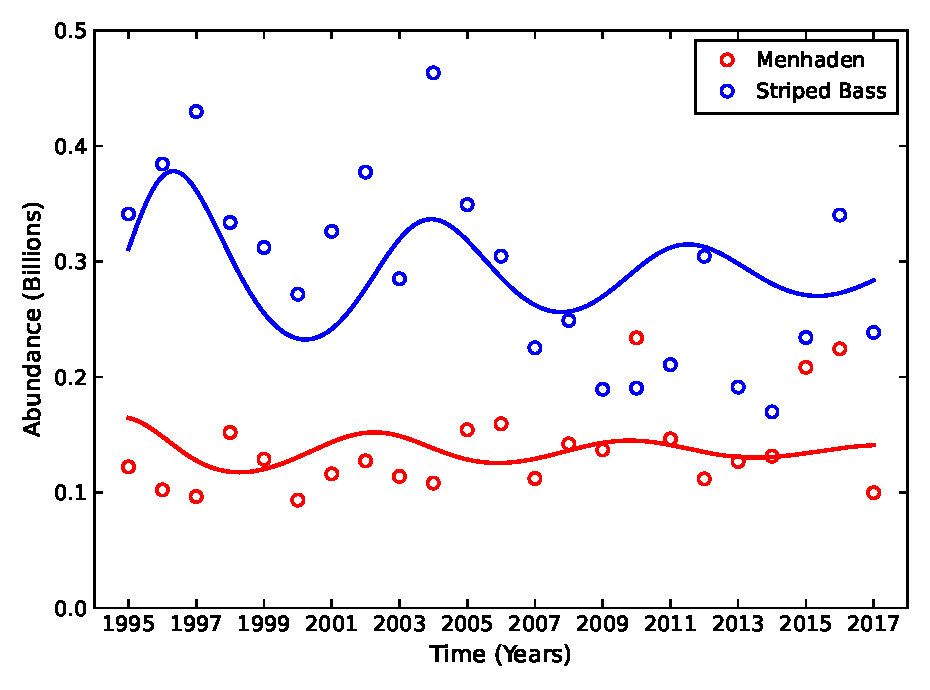
\includegraphics[width=\linewidth, keepaspectratio]{fig1_fitted_curves.pdf}
    \end{column}

    \begin{column}{0.37\textwidth}
      \begin{block}{\textbf{Quy luật dao động trễ pha}}
        \footnotesize
        \begin{enumerate}
          \item \textbf{Cá mòi dầu tăng} $\implies$ thức ăn dồi dào, thúc đẩy cá vược tăng trưởng.
          \item \textbf{Cá vược sọc tăng cao} $\implies$ áp lực săn bắt cực đại làm cá mòi sụt giảm.
          \item \textbf{Cá mòi khan hiếm} $\implies$ cá vược suy dinh dưỡng \& sụt giảm số lượng sau khoảng trễ (\textit{time lag}).
          \item Chu kỳ lặp lại tạo nên quỹ đạo dao động lệch pha sinh học.
        \end{enumerate}
      \end{block}
    \end{column}
  \end{columns}
\end{frame}

% ------------------------------------------------------------------------------
% SLIDE 14: DỰ BÁO ĐỘNG THÁI ĐẾN NĂM 2100
% ------------------------------------------------------------------------------
\begin{frame}{Dự báo động thái quần thể đến năm 2100 (Dao động tắt dần)}
  \begin{columns}[c]
    \begin{column}{0.62\textwidth}
      \centering
      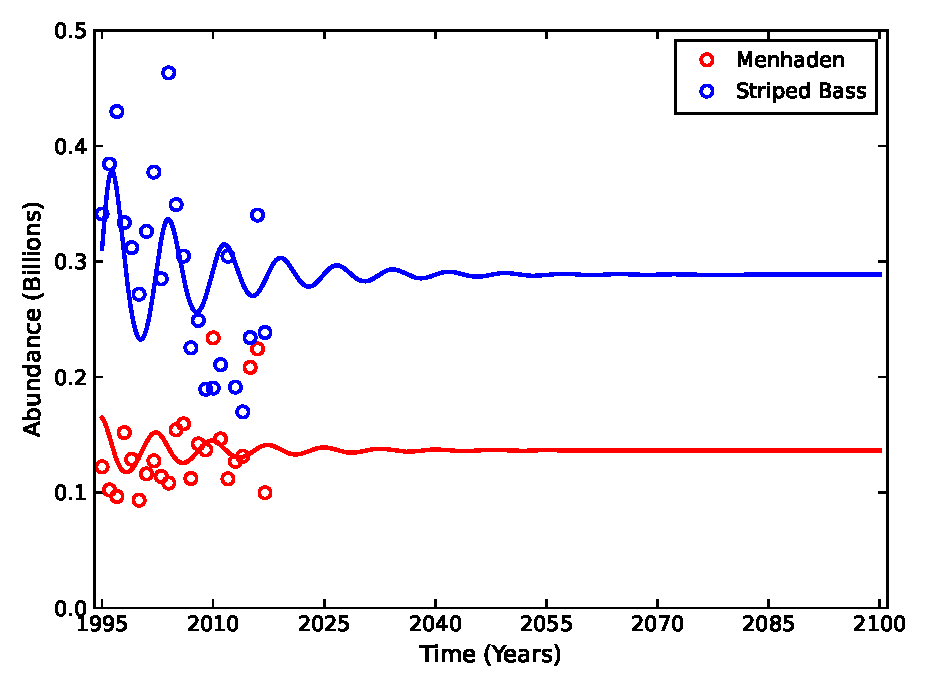
\includegraphics[width=\linewidth, keepaspectratio]{fig2_model_prediction.pdf}
    \end{column}

    \begin{column}{0.37\textwidth}
      \begin{tcolorbox}[colback=OceanLight, colframe=OceanNavy, arc=2mm, title=\textbf{Đặc điểm quỹ đạo dài hạn}]
        \footnotesize
        \begin{itemize}
          \item  Biên độ dao động giảm dần theo thời gian.
          \item  Quỹ đạo hai quần thể tiến về trạng thái cân bằng dừng tự nhiên
          $$Q = (x^*, y^*)$$
          \item Không xuất hiện tuần hoàn hay hỗn loạn.
        \end{itemize}
      \end{tcolorbox}
    \end{column}
  \end{columns}
\end{frame}

% ------------------------------------------------------------------------------
% SLIDE 15: ĐIỂM CÂN BẰNG DỪNG TỰ NHIÊN
% ------------------------------------------------------------------------------
\begin{frame}{Tính toán trạng thái cân bằng }
  \begin{block}{\textbf{Thiết lập hệ phương trình ở trạng thái cân bằng}}
    \footnotesize
    Tại điểm cân bằng  ($x^*, y^*$), đạo hàm theo thời gian bằng 0:
    \begin{equation}
    \left\{
    \begin{aligned}
    r - ax^* - by^* &= 0 \\
    -e - cy^* + dx^* &= 0
    \end{aligned}
    \right.
    \iff
    \begin{pmatrix}
    a & b \\
    -d & c
    \end{pmatrix}
    \begin{pmatrix}
    x^* \\ y^*
    \end{pmatrix}
    =
    \begin{pmatrix}
    r \\ -e
    \end{pmatrix}
    \end{equation}
  \end{block}

  \vspace{0.1cm}

  \begin{columns}[c]
    \begin{column}{0.48\textwidth}
      \begin{exampleblock}{\textbf{Công thức nghiệm tường minh (Định lý Cramer)}}
        \footnotesize
        \begin{align}
        x^* &= \frac{rc + be}{ac + bd} = \frac{2.407705}{17.661755} \approx \mathbf{0.1363} \\
        y^* &= \frac{rd - ae}{ac + bd} = \frac{5.097949}{17.661755} \approx \mathbf{0.2886}
        \end{align}
      \end{exampleblock}
    \end{column}

    \begin{column}{0.48\textwidth}
      \begin{tcolorbox}[colback=OceanLight, colframe=OceanTeal, arc=2mm, title=\textbf{Ý nghĩa thực tế cho Vịnh Chesapeake}]
        \footnotesize
        Quy đổi theo tỷ lệ chuẩn hóa $10^9$ con:
        \begin{itemize}
          \item \textbf{Cá mòi dầu:} $x^* \approx \mathbf{136.3\text{ triệu con}}$.
          \item \textbf{Cá vược sọc:} $y^* \approx \mathbf{288.6\text{ triệu con}}$.
        \end{itemize}
        Đây là trạng thái nền tảng sinh thái bền vững tự nhiên khi chưa chịu tác động đánh bắt thương mại của con người.
      \end{tcolorbox}
    \end{column}
  \end{columns}
\end{frame}

% ==============================================================================
% PHẦN 4: PHÂN TÍCH ĐỘ ĐÀN HỒI SINH THÁI (RESILIENCE) (CHƯƠNG 2)
% ==============================================================================
\section{Phân tích độ đàn hồi sinh thái}

% ------------------------------------------------------------------------------
% SLIDE 16: KHÁI NIỆM ĐỘ ĐÀN HỒI SINH THÁI
% ------------------------------------------------------------------------------
\begin{frame}{Khái niệm Độ đàn hồi sinh học (Resilience -- Pimm \& Lawton 1978)}
  \begin{columns}[t]
    \begin{column}{0.50\textwidth}
      \begin{block}{\textbf{Định nghĩa theo Pimm \& Lawton (1978)}}
        \footnotesize
        \textbf{Độ đàn hồi sinh học ($R$)} là tốc độ mà một hệ sinh thái tự ổn định và phục hồi trở về trạng thái cân bằng.
        \begin{equation}
        \tau = \frac{-1}{\mathrm{Re}(\lambda_m)} \quad \Longleftrightarrow \quad R = \frac{1}{\tau} = -\mathrm{Re}(\lambda_m)
        \end{equation}
        \begin{itemize}
          \item $\lambda_m$: Giá trị riêng có phần thực lớn nhất của ma trận Jacobian.
          \item $\tau$: Thời gian hồi phục .
        \end{itemize}
      \end{block}
    \end{column}

    \begin{column}{0.48\textwidth}
      \begin{tcolorbox}[colback=OceanLight, colframe=OceanNavy, arc=2mm, title=\textbf{Ý nghĩa cơ chế động lực học}]
        \footnotesize
        \begin{itemize}
          \item Độ đàn hồi chỉ có nghĩa khi điểm cân bằng \textbf{ổn định tiệm cận}: $\mathrm{Re}(\lambda_m) < 0$.
          \item \textbf{$R$ và $\tau$ tỷ lệ nghịch:}
          \begin{itemize}
            \item $R$ càng lớn $\implies$ $\tau$ càng nhỏ $\implies$ Hệ phục hồi nhanh, sức chống chịu cao.
            \item $R$ nhỏ $\implies$ $\tau$ lớn $\implies$ Hệ tổn thương lâu, nguy cơ suy thoái kéo dài khi gặp biến cố.
          \end{itemize}
        \end{itemize}
      \end{tcolorbox}
    \end{column}
  \end{columns}
\end{frame}

% ------------------------------------------------------------------------------
% SLIDE 17: MA TRẬN JACOBI & TÍNH ỔN ĐỊNH
% ------------------------------------------------------------------------------
\begin{frame}{Ma trận Jacobian \& Khảo sát tính ổn định tiệm cận}
  \begin{block}{\textbf{Tuyến tính hóa hệ động lực tại điểm cân bằng $Q(x^*, y^*)$}}
    \footnotesize
    Ma trận Jacobi tổng quát của hệ:
    $J(x, y) = \begin{pmatrix} r - 2ax - by & -bx \\ dy & -e - 2cy + dx \end{pmatrix}$.
    Tại điểm dừng $Q(x^*, y^*)$:
    \begin{equation}
    A = J(x^*, y^*) = \begin{pmatrix} -ax^* & -bx^* \\ dy^* & -cy^* \end{pmatrix}
    \end{equation}
  \end{block}

  \vspace{0.1cm}

  \begin{columns}[c]
    \begin{column}{0.48\textwidth}
      \begin{exampleblock}{\textbf{Vết và Định thức của ma trận $A$}}
        \footnotesize
        \begin{align}
        \mathrm{tr}(A) &= -(ax^* + cy^*) < 0 \\
        \det(A) &= (ac + bd)x^*y^* > 0
        \end{align}
      \end{exampleblock}
    \end{column}

    \begin{column}{0.48\textwidth}
      \begin{tcolorbox}[colback=OceanLight, colframe=OceanTeal, arc=2mm, title=\textbf{Tiêu chuẩn Routh--Hurwitz}]
        \footnotesize
        Do $\mathrm{tr}(A) < 0$ và $\det(A) > 0$, mọi giá trị riêng của $A$ đều có \textbf{phần thực âm} $\implies$ Trạng thái cân bằng đồng tồn tại $Q$ là \textbf{ổn định tiệm cận cục bộ} (\textit{locally asymptotically stable}).
      \end{tcolorbox}
    \end{column}
  \end{columns}
\end{frame}

% ------------------------------------------------------------------------------
% SLIDE 18: GIÁ TRỊ RIÊNG & THỜI GIAN PHỤC HỒI
% ------------------------------------------------------------------------------
\begin{frame}{Tính toán giá trị riêng \& Thời gian hồi phục của Vịnh Chesapeake}
  \begin{block}{\textbf{Thay thế số liệu cụ thể vào phương trình đặc trưng}}
    \footnotesize
    Phương trình đặc trưng: $\det(\lambda I - A) = \lambda^2 - \mathrm{tr}(A)\lambda + \det(A) = 0$.
    \begin{itemize}
      \item $\mathrm{tr}(A) = -[(0.026)(0.1363) + (0.520)(0.2886)] = \mathbf{-0.1536158}$
      \item $\det(A) = (17.661755)(0.1363)(0.2886) \approx \mathbf{0.694747}$
      \item Biệt thức: $\Delta = (\mathrm{tr}(A))^2 - 4\det(A) = (-0.1536)^2 - 4(0.6947) = \mathbf{-2.75539} < 0$
    \end{itemize}
  \end{block}

  \vspace{0.1cm}

  \begin{columns}[c]
    \begin{column}{0.48\textwidth}
      \begin{exampleblock}{\textbf{Cặp giá trị riêng phức liên hợp}}
        \footnotesize
        \begin{equation}
        \lambda_{1, 2} \approx \mathbf{-0.0768 \pm 0.8301i}
        \end{equation}
        Trùng khớp chính xác với công thức (2) trong bài báo gốc của Panayotova et al. (2023).
      \end{exampleblock}
    \end{column}

    \begin{column}{0.48\textwidth}
      \begin{tcolorbox}[colback=OceanLight, colframe=OceanNavy, arc=2mm, title=\textbf{Độ đàn hồi \& Thời gian hồi phục}]
        \footnotesize
        \begin{align}
        R &= -\mathrm{Re}(\lambda_m) \approx \mathbf{0.0768\text{ năm}^{-1}} \\[2pt]
        \tau &= \frac{1}{R} \approx \frac{1}{0.0768} \approx \mathbf{13.021\text{ năm}}
        \end{align}
      \end{tcolorbox}
    \end{column}
  \end{columns}
\end{frame}


% ==============================================================================
% PHẦN 4: MÔ HÌNH SINH HỌC--KINH TẾ VÀ PHÂN TÍCH ỔN ĐỊNH (CHƯƠNG 3)
% ==============================================================================
\section{Mô hình sinh học--kinh tế \& Phân tích ổn định }

% ------------------------------------------------------------------------------
% SLIDE 20: MÔ HÌNH SINH HỌC--KINH TẾ MỞ RỘNG (CHƯƠNG 3)
% ------------------------------------------------------------------------------
\begin{frame}{Mô hình sinh học--kinh tế mở rộng }
  \begin{columns}[c]
    \begin{column}{0.48\textwidth}
      \begin{block}{\textbf{Hệ phương trình vi phân có khai thác}}
        \footnotesize
        Mở rộng mô hình Lotka--Volterra bằng cách bổ sung hoạt động khai thác của con người:
        \begin{equation}
        \label{eq:ch3_bionomic_system}
        \left\{
        \begin{aligned}
        \frac{dx}{dt} &= x(r - ax - by) - q_1 E_1 x, \\
        \frac{dy}{dt} &= y(-e - cy + dx) - q_2 E_2 y.
        \end{aligned}
        \right.
        \end{equation}
        $\bullet$ \textbf{Giả thiết CPUE} (\textit{Catch Per Unit Effort}):\\
        Sản lượng đánh bắt trên một đơn vị thời gian:
        $$h_1 = q_1 E_1 x, \qquad h_2 = q_2 E_2 y$$
      \end{block}
    \end{column}

    \begin{column}{0.50\textwidth}
      \begin{block}{\textbf{Hàm lợi nhuận kinh tế ròng ($\pi$)}}
        \footnotesize
        Tổng lợi nhuận từ hoạt động khai thác hải sản:
        $$\pi(E_1, E_2) = (p_1 q_1 x - c_1)E_1 + (p_2 q_2 y - c_2)E_2$$
        $\bullet$ Doanh thu: $p_1 q_1 E_1 x + p_2 q_2 E_2 y$\\
        $\bullet$ Chi phí: $c_1 E_1 + c_2 E_2$
      \end{block}

      \vspace{0.1cm}

      \begin{tcolorbox}[colback=OceanLight, colframe=OceanNavy, arc=1.5mm, top=1.2mm, bottom=1.2mm, title={\textbf{Ý nghĩa các tham số kinh tế}}]
        \footnotesize
        $\bullet$ $E_1, E_2$: Cường độ khai thác Menhaden và Bass.\\
        $\bullet$ $q_1, q_2$: Hệ số khả năng đánh bắt (\textit{catchability}).\\
        $\bullet$ $p_1, p_2$: Giá bán trên một đơn vị sinh khối.\\
        $\bullet$ $c_1, c_2$: Chi phí trên đơn vị nỗ lực khai thác.
      \end{tcolorbox}
    \end{column}
  \end{columns}
\end{frame}

% ------------------------------------------------------------------------------
% SLIDE 21: TÍNH CHẤT ĐỊNH TÍNH CỦA NGHIỆM: TÍNH KHÔNG ÂM & BỊ CHẶN
% ------------------------------------------------------------------------------
\begin{frame}{Tính chất định tính của nghiệm: Tính không âm \& Bị chặn}
  \vspace*{-0.25cm}
  \begin{columns}[c]
    \begin{column}{0.48\textwidth}
      \begin{block}{\textbf{1. Tính không âm của quần thể ($x, y \ge 0$)}}
        \footnotesize
        Tích phân hệ vi phân cho nghiệm dạng mũ ($x_0, y_0 > 0$):\\
        $\bullet$ $x(t) = x(0)\exp\left(\int_0^t [r - ax - by - q_1 E_1]\,ds\right) \ge 0$\\
        $\bullet$ $y(t) = y(0)\exp\left(\int_0^t [-e - cy + dx - q_2 E_2]\,ds\right) \ge 0$\\[1pt]
        $\implies$ Quần thể luôn dương trong miền $\mathbb{R}^2_+$ với mọi $t \ge 0$.
      \end{block}

      \vspace{0.05cm}

      \begin{block}{\textbf{2. Tính bị chặn toàn cục \& Miền $\Omega$}}
        \footnotesize
        $\bullet$ Đặt $w(t) = x(t) + \frac{y(t)}{\gamma}$ với $\gamma = \frac{d}{b}$.\\
        $\bullet$ Bất đẳng thức: $\frac{dw}{dt} + \delta w \le \frac{r^2}{4a}$ ($\delta = \min\{q_1 E_1, q_2 E_2, e\}$).\\
        $\bullet$ Lấy tích phân $\implies \limsup_{t \to \infty} w(t) \le L = \frac{r^2}{4a\delta}$.\\[1pt]
        $\implies$ Quần thể bị chặn trong miền bất biến:
        $$\Omega = \left\{ (x, y) \in \mathbb{R}^2_+ \;\middle|\; x \le \frac{r}{a}, \; x + \frac{y}{\gamma} \le L \right\}$$
      \end{block}
    \end{column}

    \begin{column}{0.50\textwidth}
      \centering
      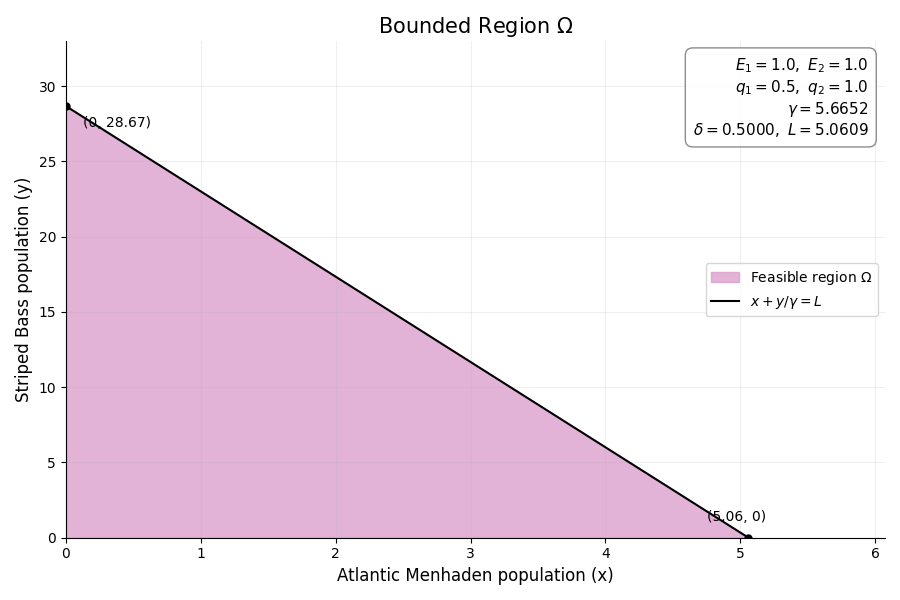
\includegraphics[width=\linewidth, height=4.1cm, keepaspectratio]{pictures/ch3/region_omega.png}\\[3pt]
      {\scriptsize \textit{Hình 3.1: Minh họa miền bất biến sinh thái $\Omega$ của hệ thống}}
    \end{column}
  \end{columns}
\end{frame}

% ------------------------------------------------------------------------------
% SLIDE 22: XÁC ĐỊNH CÁC ĐIỂM CÂN BẰNG SINH HỌC--KINH TẾ
% ------------------------------------------------------------------------------
\begin{frame}{Xác định các điểm cân bằng sinh học--kinh tế}
  \vspace*{-0.25cm}
  \begin{block}{\textbf{Điều kiện cân bằng sinh học--kinh tế (Bionomic Equilibrium)}}
    \footnotesize
    Trạng thái dừng động học quần thể đồng thời lợi nhuận kinh tế triệt tiêu:
    $\frac{dx}{dt} = 0, \quad \frac{dy}{dt} = 0, \quad \pi(E_1, E_2) = 0$.
  \end{block}

  \vspace{0.05cm}

  \begin{center}
  \scriptsize
  \renewcommand{\arraystretch}{1.02}
  \begin{tabularx}{\textwidth}{l X X}
    \toprule
    \textbf{Trường hợp} & \textbf{Tọa độ điểm cân bằng} & \textbf{Điều kiện tồn tại} \\
    \midrule
    \textbf{$P_1$:} Chỉ bắt Bass & $x_B = \frac{r}{a} - \frac{bc_2}{ap_2q_2}, \quad y_B = \frac{c_2}{p_2q_2}$ & $\frac{r}{a} > \frac{bc_2}{ap_2q_2}$ \\
    ($E_1 = 0, E_2 > 0$) & $E_{2B} = -\frac{e}{q_2} - \frac{cc_2}{p_2q_2^2} + \frac{d}{q_2}\left(\frac{r}{a} - \frac{bc_2}{ap_2q_2}\right)$ & và $E_{2B} > 0$ \\
    \midrule
    \textbf{$P_2$:} Chỉ bắt Menhaden & $x_B = \frac{c_1}{p_1q_1}, \quad y_B = \frac{dc_1}{cp_1q_1} - \frac{e}{c}$ & $\frac{dc_1}{cp_1q_1} > \frac{e}{c}$ \\
    ($E_1 > 0, E_2 = 0$) & $E_{1B} = \frac{r}{q_1} - \frac{ac_1}{p_1q_1^2} - \frac{b}{q_1}\left(\frac{dc_1}{cp_1q_1} - \frac{e}{c}\right)$ & và $E_{1B} > 0$ \\
    \midrule
    \textbf{$P_3$:} Không khai thác & $x^* = \frac{rc+be}{ac+bd}, \quad y^* = \frac{rd-ae}{ac+bd}$ & $rd > ae$ \\
    ($E_1 = 0, E_2 = 0$) & (Trạng thái cân bằng dừng tự nhiên $Q$) & (Điểm dừng sinh thái) \\
    \midrule
    \textbf{$P_4$:} Khai thác cả 2 loài & $x_B = \frac{c_1}{p_1q_1}, \quad y_B = \frac{c_2}{p_2q_2}$ & $E_{1B} > 0$ \\
    ($E_1 > 0, E_2 > 0$) & $E_{1B}, E_{2B}$ tính tường minh từ hệ Cramer & và $E_{2B} > 0$ \\
    \bottomrule
  \end{tabularx}
  \end{center}
\end{frame}

% ------------------------------------------------------------------------------
% SLIDE 23: PHÂN TÍCH TÍNH ỔN ĐỊNH & NGƯỠNG KHAI THÁC TỚI HẠN
% ------------------------------------------------------------------------------
\begin{frame}{Phân tích tính ổn định \& Ngưỡng khai thác tới hạn ($E_{\mathrm{crit}}$)}
  \begin{columns}[t]
    \begin{column}{0.48\textwidth}
      \begin{block}{\textbf{Ma trận Jacobian dưới khai thác}}
        \footnotesize
        Tại điểm cân bằng cùng tồn tại $(\hat{x}, \hat{y})$:
        $$J(\hat{x}, \hat{y}) = \begin{pmatrix} -a\hat{x} & -b\hat{x} \\ d\hat{y} & -c\hat{y} \end{pmatrix}$$
        $\bullet$ Vết ma trận:
        $$\operatorname{tr}(J) = -(a\hat{x} + c\hat{y}) < 0$$
        $\bullet$ Định thức:
        $$\det(J) = (ac + bd)\hat{x}\hat{y} > 0$$
      \end{block}

      \vspace{0.1cm}

      \begin{exampleblock}{\textbf{Tiêu chuẩn Routh--Hurwitz}}
        \footnotesize
        $\operatorname{tr}(J) < 0$ và $\det(J) > 0 \implies$ Mọi trị riêng có phần thực âm.\\
        $\implies$ Điểm cân bằng cùng tồn tại $(\hat{x}, \hat{y})$ \textbf{luôn ổn định tiệm cận} trong miền tồn tại.
      \end{exampleblock}
    \end{column}

    \begin{column}{0.50\textwidth}
      \begin{alertblock}{\textbf{Ngưỡng khai thác tới hạn ($E_{\mathrm{crit}}$)}}
        \footnotesize
        Điều kiện để cá vược không bị tuyệt chủng ($\hat{y} > 0$):
        \begin{itemize}
          \setlength{\itemsep}{2pt}
          \item \textbf{Chỉ bắt Bass:} $E_2 < E_{2,\mathrm{crit}} = \frac{rd - ae}{aq_2} \approx \mathbf{196.8}$
          \item \textbf{Chỉ bắt Menhaden:} $E_1 < E_{1,\mathrm{crit}} = \frac{rd - ae}{dq_1} \approx \mathbf{1.02}$
          \item \textbf{Bắt đồng thời:} $E < E_{\mathrm{crit}} = \frac{rd - ae}{dq_1 + aq_2} \approx \mathbf{1.015}$
        \end{itemize}
      \end{alertblock}

      \vspace{0.1cm}

      \begin{tcolorbox}[colback=OceanLight, colframe=OceanNavy, arc=1.5mm, top=1.2mm, bottom=1.2mm]
        \footnotesize
        Khi $E \to E_{\mathrm{crit}}^-$, thời gian phục hồi $\tau(E) \to +\infty$ (sụp đổ sức chống chịu của hệ sinh thái).
      \end{tcolorbox}
    \end{column}
  \end{columns}
\end{frame}

% ------------------------------------------------------------------------------
% SLIDE 24: MINH HỌA SỐ: CHÂN DUNG PHA DƯỚI 4 CHẾ ĐỘ KHAI THÁC
% ------------------------------------------------------------------------------
\begin{frame}{Minh họa số: Chân dung pha dưới 4 chế độ khai thác}
  \begin{columns}[c]
    \begin{column}{0.56\textwidth}
      \centering
      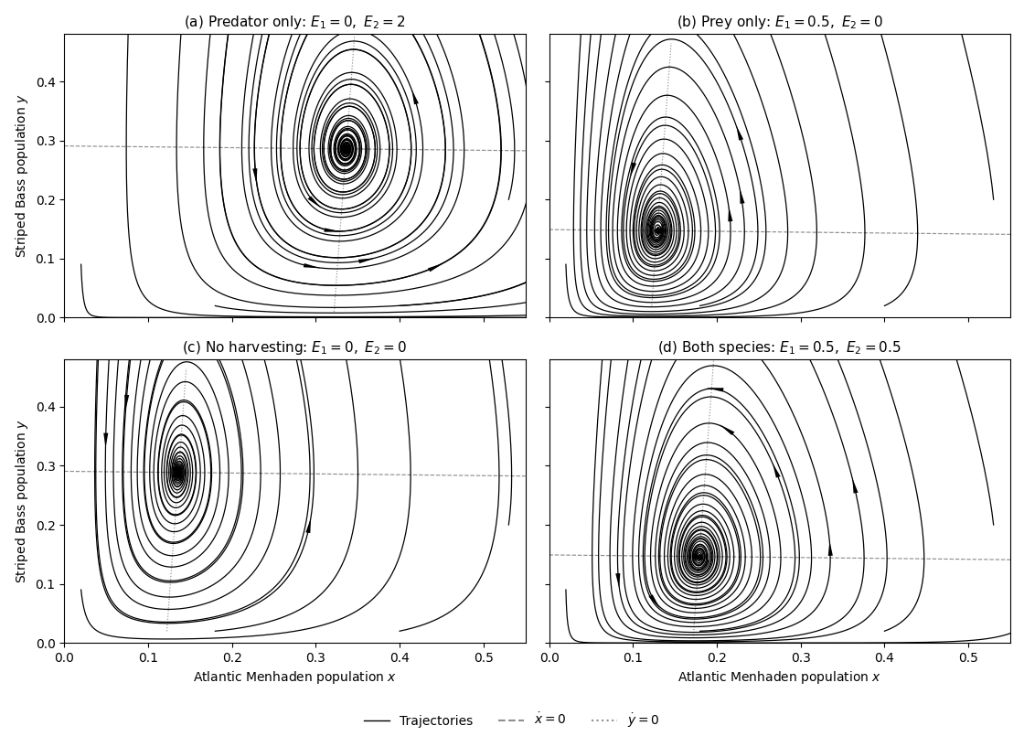
\includegraphics[width=\linewidth, height=4.6cm, keepaspectratio]{pictures/ch3/phase_potrait.png}\\[3pt]
      {\scriptsize \textit{Hình 3.2: Chân dung pha: (a) chỉ bắt Bass; (b) chỉ bắt Menhaden; (c) không khai thác; (d) bắt đồng thời}}
    \end{column}

    \begin{column}{0.42\textwidth}
      \begin{block}{\textbf{Đặc điểm quỹ đạo nghiệm}}
        \footnotesize
        $\bullet$ Quỹ đạo xoắn ốc hội tụ về điểm cân bằng cùng tồn tại $(\hat{x}, \hat{y})$ từ mọi điều kiện ban đầu $x(0) > 0, y(0) > 0$.\\
        $\bullet$ Minh chứng trực quan tính \textbf{ổn định tiệm cận} của hệ động lực dưới khai thác.
      \end{block}

      \vspace{0.1cm}

      \begin{exampleblock}{\textbf{Dịch chuyển tâm cân bằng}}
        \footnotesize
        $\bullet$ \textbf{Khai thác Bass (a):} Tâm xoắn dịch sang phải (sinh khối Menhaden tăng do giảm săn bắt).\\
        $\bullet$ \textbf{Khai thác Menhaden (b):} Tâm xoắn dịch mạnh xuống dưới (Bass cạn thức ăn).
      \end{exampleblock}
    \end{column}
  \end{columns}
\end{frame}

% ------------------------------------------------------------------------------
% SLIDE 25: MINH HỌA SỐ: THỜI GIAN HỒI PHỤC THEO CƯỜNG ĐỘ KHAI THÁC
% ------------------------------------------------------------------------------
\begin{frame}{Minh họa số: Thời gian hồi phục $\tau$ theo cường độ khai thác}
  \begin{columns}[c]
    \begin{column}{0.56\textwidth}
      \centering
      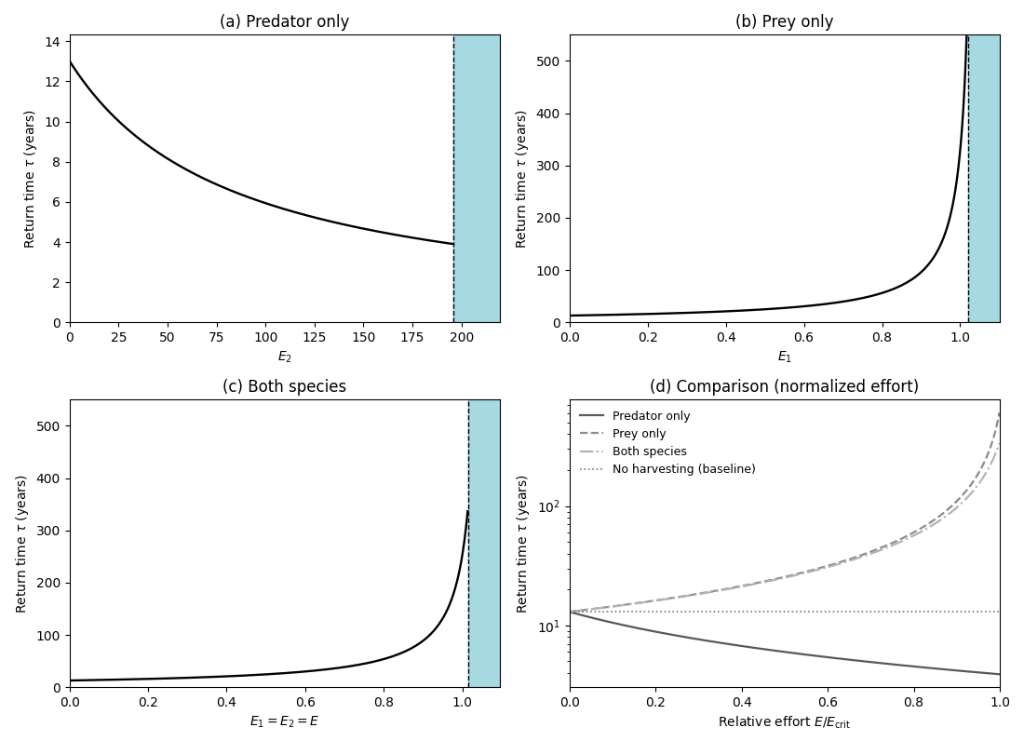
\includegraphics[width=\linewidth, height=4.6cm, keepaspectratio]{pictures/ch3/return_time.png}\\[3pt]
      {\scriptsize \textit{Hình 3.3: Thời gian hồi phục $\tau$: (a) chỉ Bass; (b) chỉ Menhaden; (c) đồng thời; (d) đường chuẩn hóa}}
    \end{column}

    \begin{column}{0.42\textwidth}
      \begin{block}{\textbf{Quy luật biến thiên của $\tau$}}
        \footnotesize
        $\bullet$ \textbf{Chỉ bắt Bass (a):} $\tau$ ban đầu giảm (nhờ giảm cạnh tranh nội bộ bãi đẻ), sau đó tăng vọt tới vô hạn khi $E_2 \to E_{2,\mathrm{crit}}$.\\
        $\bullet$ \textbf{Chỉ bắt Menhaden (b) \& Đồng thời (c):} $\tau$ tăng đơn điệu ngay từ đầu và bùng nổ tới $+\infty$ khi chạm $E_{\mathrm{crit}} \approx 1.02$.
      \end{block}

      \vspace{0.1cm}

      \begin{alertblock}{\textbf{Vùng tuyệt chủng (Màu xanh)}}
        \footnotesize
        Khi vượt quá $E_{\mathrm{crit}}$, Striped Bass bị tuyệt chủng hoàn toàn, liên kết 2 loài bị phá vỡ.
      \end{alertblock}
    \end{column}
  \end{columns}
\end{frame}

% ==============================================================================
% PHẦN 5: PHÂN TÍCH CÁC CHÍNH SÁCH KHAI THÁC NGHỀ CÁ (CHƯƠNG 4)
% ==============================================================================
\section{Chính sách khai thác nghề cá (Chương 4)}

% ------------------------------------------------------------------------------
% SLIDE 20: CHÍNH SÁCH SẢN LƯỢNG BỀN VỮNG TỐI ĐA (MSY)
% ------------------------------------------------------------------------------
\begin{frame}{Chính sách Sản lượng bền vững tối đa (MSY)}
  \begin{columns}[t]
    \begin{column}{0.49\textwidth}
      \begin{block}{\textbf{1. Chỉ khai thác cá vược ($E_1 = 0, E_2 = E$)}}
        \scriptsize
        $\bullet$ Sản lượng: $Y(E) = \frac{E(rd - ae - aq_2 E)}{ac + bd}$.\\
        $\bullet$ Cực đại: $E_{\mathrm{MSY}} = \frac{rd - ae}{2aq_2} \approx 98.4$ ($q_2 = 1$).\\
        $\bullet$ Quần thể bass ở mức MSY bằng \textbf{50\%} khi chưa đánh bắt $\implies$ Hai loài đồng tồn tại bền vững.
      \end{block}
      
      \vspace{0.05cm}
      \centering
      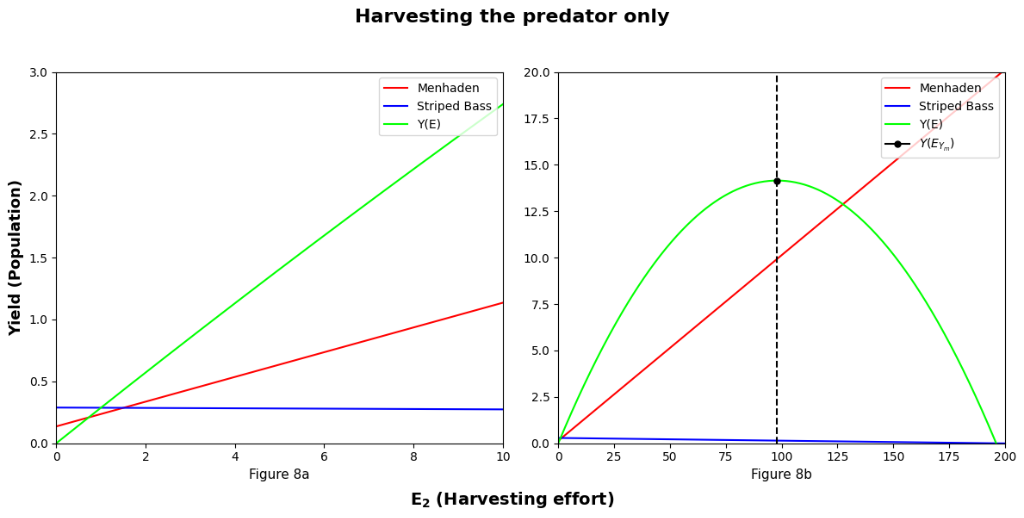
\includegraphics[height=2.3cm, keepaspectratio]{pictures/ch4/fig8_msy_predator.png}\\[1pt]
      {\tiny \textit{Hình 8: Chỉ khai thác bass ($E_2$)}}
    \end{column}

    \begin{column}{0.49\textwidth}
      \begin{alertblock}{\textbf{2. Chỉ khai thác cá mòi ($E_1 = E, E_2 = 0$)}}
        \scriptsize
        $\bullet$ Cực đại toán học: $E_{Ym} = \frac{cr + be}{2cq_1} \approx 4.6$.\\
        $\bullet$ \textbf{Cảnh báo tuyệt chủng:} Điều kiện $\frac{rd-ae}{cr+be} > \frac{d}{2c}$ không thỏa mãn; cá vược tuyệt chủng khi $E > 1.02$!\\
        $\blacktriangleright$ \textbf{Khuyến nghị an toàn:} $E_{\mathrm{MSY}} = 0.5$ (giảm 50\% nỗ lực).
      \end{alertblock}

      \vspace{0.05cm}
      \centering
      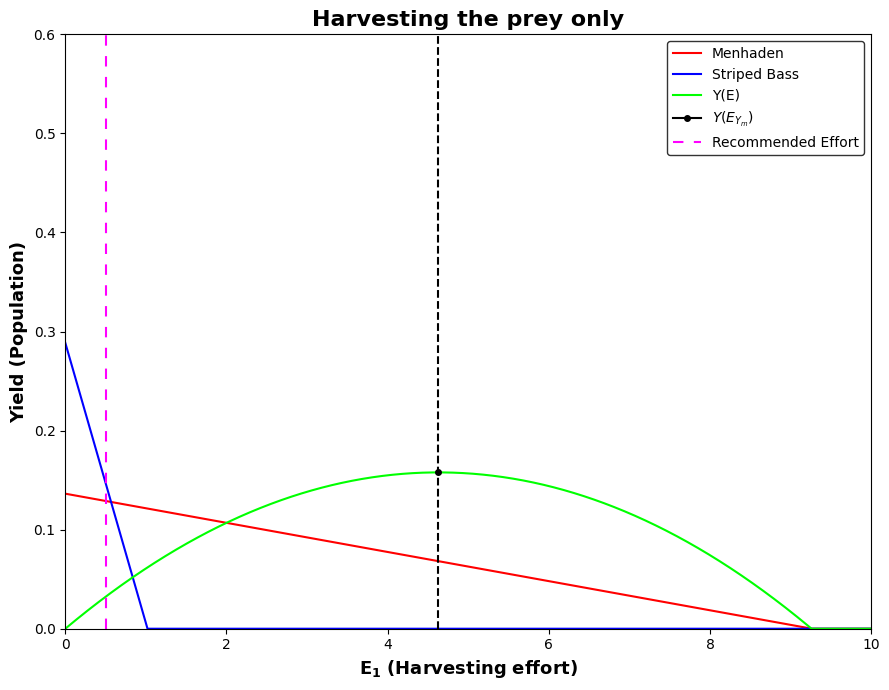
\includegraphics[height=2.3cm, keepaspectratio]{pictures/ch4/fig9_msy_prey.png}\\[1pt]
      {\tiny \textit{Hình 9: Chỉ khai thác menhaden ($E_1$)}}
    \end{column}
  \end{columns}
\end{frame}

% ------------------------------------------------------------------------------
% SLIDE 21: KHAI THÁC KẾT HỢP HAI LOÀI & CHÍNH SÁCH MEY
% ------------------------------------------------------------------------------
\begin{frame}{Khai thác kết hợp hai loài \& Chính sách MEY}
  \begin{columns}[t]
    \begin{column}{0.49\textwidth}
      \begin{block}{\textbf{Khai thác đồng thời 2 loài ($E_1 = E_2 = E$)}}
        \scriptsize
        $\bullet$ Tổng sản lượng: $Y(E) = E(q_1\hat{x} + q_2\hat{y})$.\\
        $\bullet$ Ngưỡng an toàn để cá vược còn tồn tại:
        $$E < \frac{rd - ae}{dq_1 + aq_2} \approx 1.0146 \quad (q_1=0.5, q_2=1)$$
        $\bullet$ Cực đại toán học làm suy kiệt cá vược $\implies$ Khuyến nghị thận trọng: \textbf{$E_{\mathrm{MSY}} = 0.5$}.
      \end{block}

      \vspace{0.05cm}
      \centering
      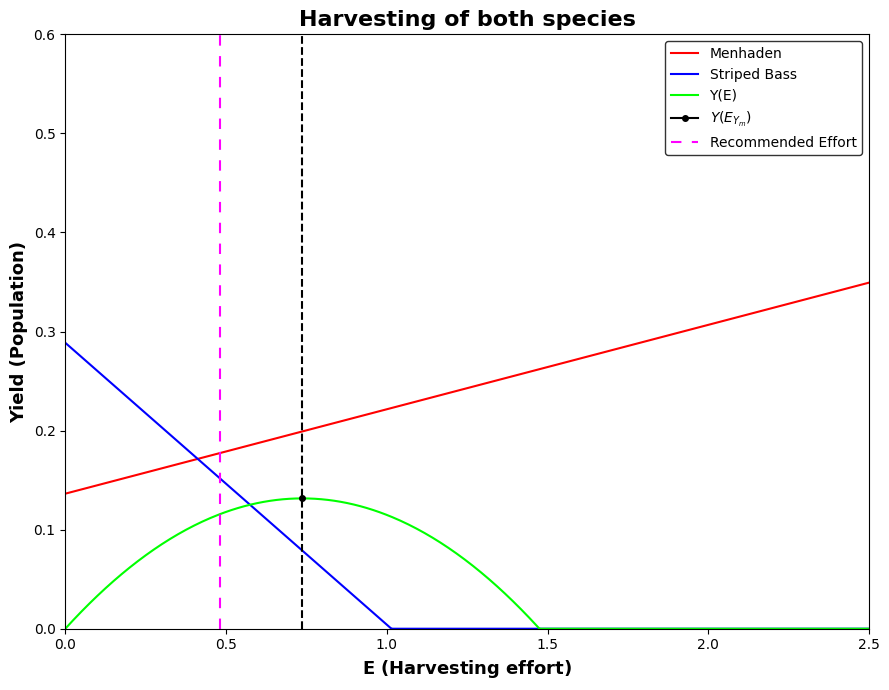
\includegraphics[height=2.0cm, keepaspectratio]{pictures/ch4/fig10_msy_combined.png}\\[1pt]
      {\tiny \textit{Hình 10: Khai thác đồng thời menhaden \& bass}}
    \end{column}

    \begin{column}{0.49\textwidth}
      \begin{tcolorbox}[colback=OceanLight, colframe=OceanNavy, arc=1.5mm, title={\textbf{Sản lượng kinh tế tối đa (MEY)}}]
        \scriptsize
        $\bullet$ Hàm tô kinh tế: $\operatorname{Rent}(E) = \hat{p}Y(E) - \hat{c}E$.\\[2pt]
        $\bullet$ \textbf{Chỉ bắt cá vược sọc:}
        $$E_{\mathrm{MEY}} = E_{\mathrm{MSY}} - \frac{\hat{c}(ac+bd)}{2\hat{p}aq_2} < E_{\mathrm{MSY}}$$
        $\implies$ \textbf{MEY thân thiện với bảo tồn hơn MSY!}\\[2pt]
        $\bullet$ \textbf{Bắt cá mòi hoặc cả 2 loài:} Dưới giả định chuẩn ($\hat{p}=2\hat{c}$), $E_{\mathrm{MEY}} < 0$.\\
        $\implies$ Thị trường tự do không tự điều tiết, cần chính sách hỗ trợ bảo tồn.
      \end{tcolorbox}
    \end{column}
  \end{columns}
\end{frame}

% ------------------------------------------------------------------------------
% SLIDE 22A: CHÍNH SÁCH RMY - CHỈ KHAI THÁC CÁ VƯỢC (BASS)
% ------------------------------------------------------------------------------
\begin{frame}{Chính sách RMY: Kịch bản chỉ khai thác cá vược ($E_1 = 0, E_2 = E$)}
  \vspace*{-0.15cm}
  \begin{block}{\textbf{Mục tiêu RMY \& Động thái hồi phục sinh thái}}
    \footnotesize
    $\bullet$ \textbf{Mục tiêu RMY:} Tối đa hóa tốc độ phục hồi hệ thống: $R(E) = 1/\tau = -\operatorname{Re}(\lambda_m)$.\\[2pt]
    $\bullet$ \textbf{Quy luật:} $R$ tăng tuyến tính theo nỗ lực khai thác cá vược $\implies E_{\mathrm{RMY}} = 10$.\\
    $\bullet$ \textbf{Cơ chế:} Đánh bắt cá vược làm giảm cạnh tranh nội bộ bãi đẻ, thúc đẩy tốc độ hồi phục toàn vịnh.
  \end{block}

  \vspace{0.08cm}
  \centering
  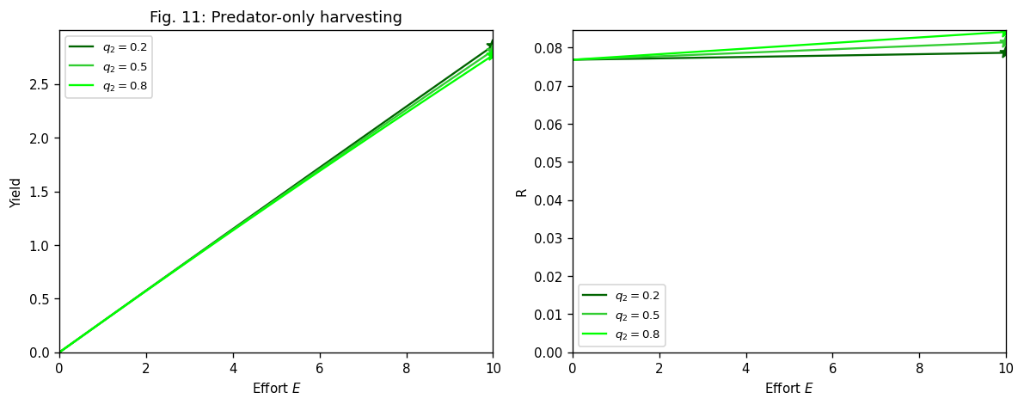
\includegraphics[width=0.86\textwidth, height=4.2cm, keepaspectratio]{pictures/ch4/fig11_rmy_predator.png}\\[2pt]
  {\scriptsize \textit{Hình 11: Đường cong sản lượng và Độ đàn hồi sinh thái $R$ theo nỗ lực $E$ khi chỉ đánh bắt cá vược}}
\end{frame}

% ------------------------------------------------------------------------------
% SLIDE 22B: CHÍNH SÁCH RMY - KHAI THÁC CÁ MÒI HOẶC CẢ 2 LOÀI
% ------------------------------------------------------------------------------
\begin{frame}{Chính sách RMY: Kịch bản khai thác cá mòi hoặc cả 2 loài}
  \vspace*{-0.15cm}
  \begin{alertblock}{\textbf{Cảnh báo sụp đổ độ đàn hồi sinh thái khi đánh bắt cá mòi dầu ($E_1 > 0$)}}
    \footnotesize
    $\bullet$ \textbf{Quy luật:} Tốc độ hồi phục $R$ \textbf{giảm nghiêm ngặt} theo nỗ lực đánh bắt cá mòi $\implies E_{\mathrm{RMY}} = 0$.\\[2pt]
    $\bullet$ \textbf{Nguy cơ tuyệt chủng:} Đánh bắt cá mòi làm cạn kiệt thức ăn của cá vược. Khi $E_1 \ge E_{\mathrm{crit}} \approx 1.02$, cá vược tuyệt chủng và $R = 0$ (đoạn đứt nét trên đồ thị).\\
    $\blacktriangleright$ \textbf{Khuyến nghị RMY:} Tuyệt đối không đánh bắt cá mòi ở mức tối đa để bảo toàn sức chống chịu sinh thái.
  \end{alertblock}

  \vspace{0.08cm}
  \centering
  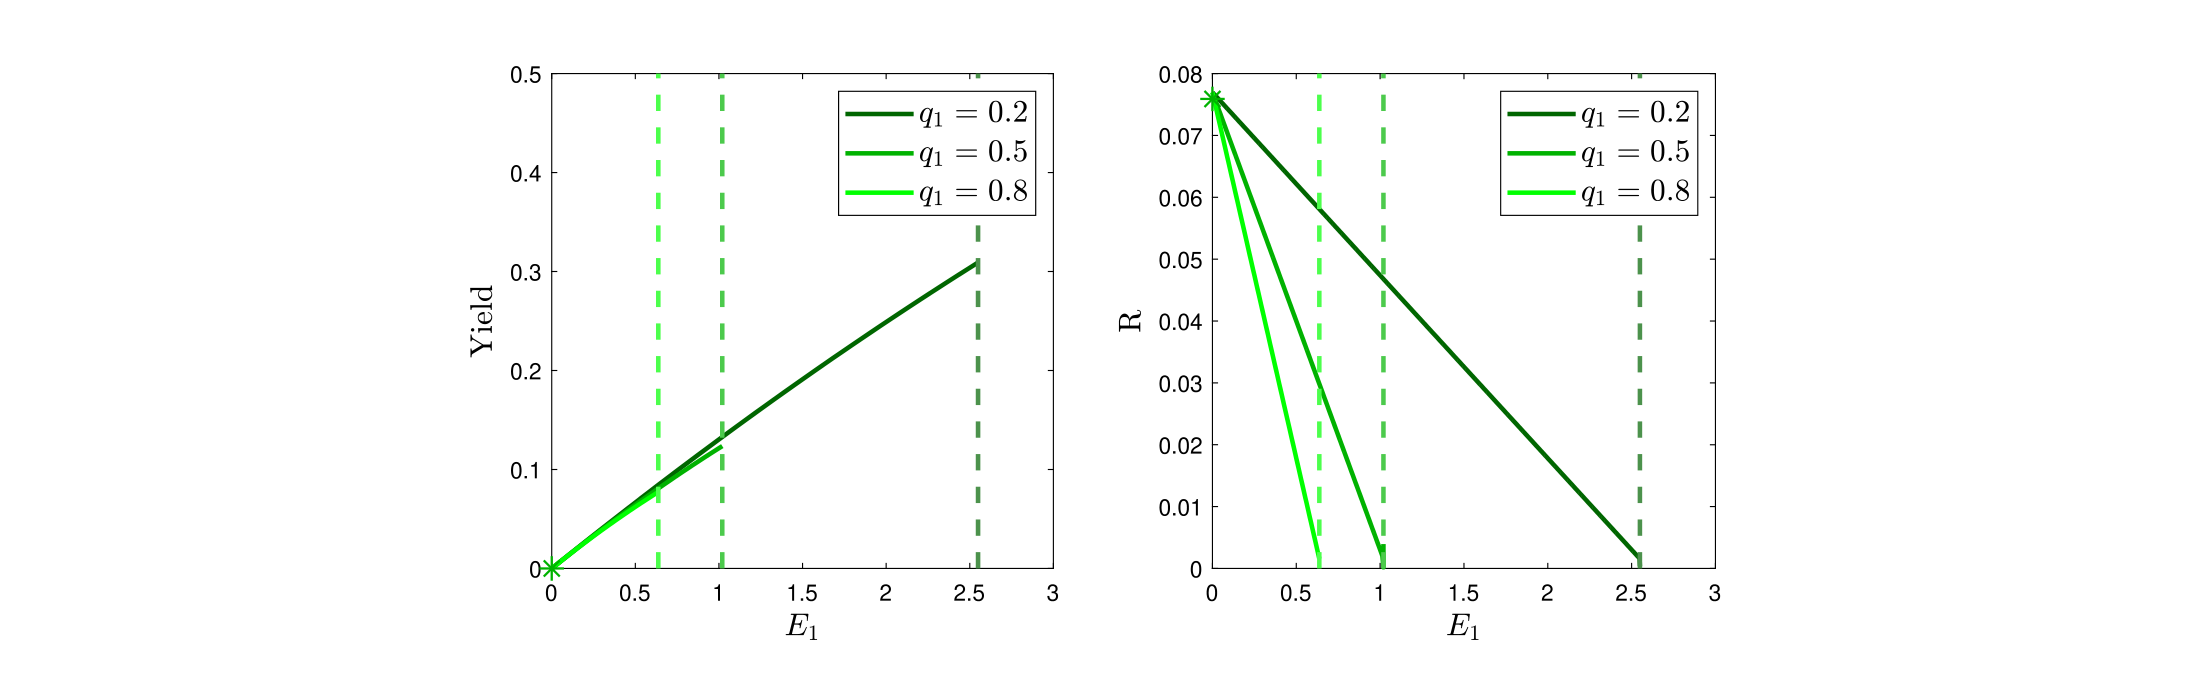
\includegraphics[width=0.86\textwidth, height=4.2cm, keepaspectratio]{pictures/ch4/fig12_rmy_prey.png}\\[2pt]
  {\scriptsize \textit{Hình 12: Sản lượng và Độ đàn hồi sinh thái $R$ khi đánh bắt cá mòi (đường đứt đoạn biểu thị cá vược tuyệt chủng)}}
\end{frame}

% ==============================================================================
% PHẦN 5: PHÂN TÍCH ĐỘ NHẠY CỤC BỘ (CHƯƠNG 5)
% ==============================================================================
\section{Phân tích độ nhạy cục bộ (Chương 5)}

% ------------------------------------------------------------------------------
% SLIDE 23: PHƯƠNG PHÁP VI PHÂN TRỰC TIẾP (DDM)
% ------------------------------------------------------------------------------
\begin{frame}{Phân tích độ nhạy cục bộ: Phương pháp vi phân trực tiếp (DDM)}
  \begin{columns}[c]
    \begin{column}{0.48\textwidth}
      \begin{block}{\textbf{Hệ 18 phương trình vi phân}}
        \scriptsize
        $\bullet$ Vector trạng thái: $u = (x, y)^\mathsf{T}$.\\
        $\bullet$ Vector 8 tham số:\\
        $p = (r, a, b, E_1, e, c, d, E_2)$.\\[2pt]
        $\bullet$ PT vi phân đạo hàm độ nhạy:
        $$\frac{d}{dt}\left(\frac{\partial u}{\partial p_j}\right) = J(u) S_j + F_j$$
        $\bullet$ $J(u) = \partial f/\partial u$ (Jacobian hệ thống).\\
        $\bullet$ $F_j = \partial f/\partial p_j$ (đạo hàm riêng theo tham số).\\
        $\bullet$ Tích phân đồng thời 2 PT trạng thái + 16 PT độ nhạy theo thời gian (1995--2100).
      \end{block}
    \end{column}

    \begin{column}{0.51\textwidth}
      \centering
      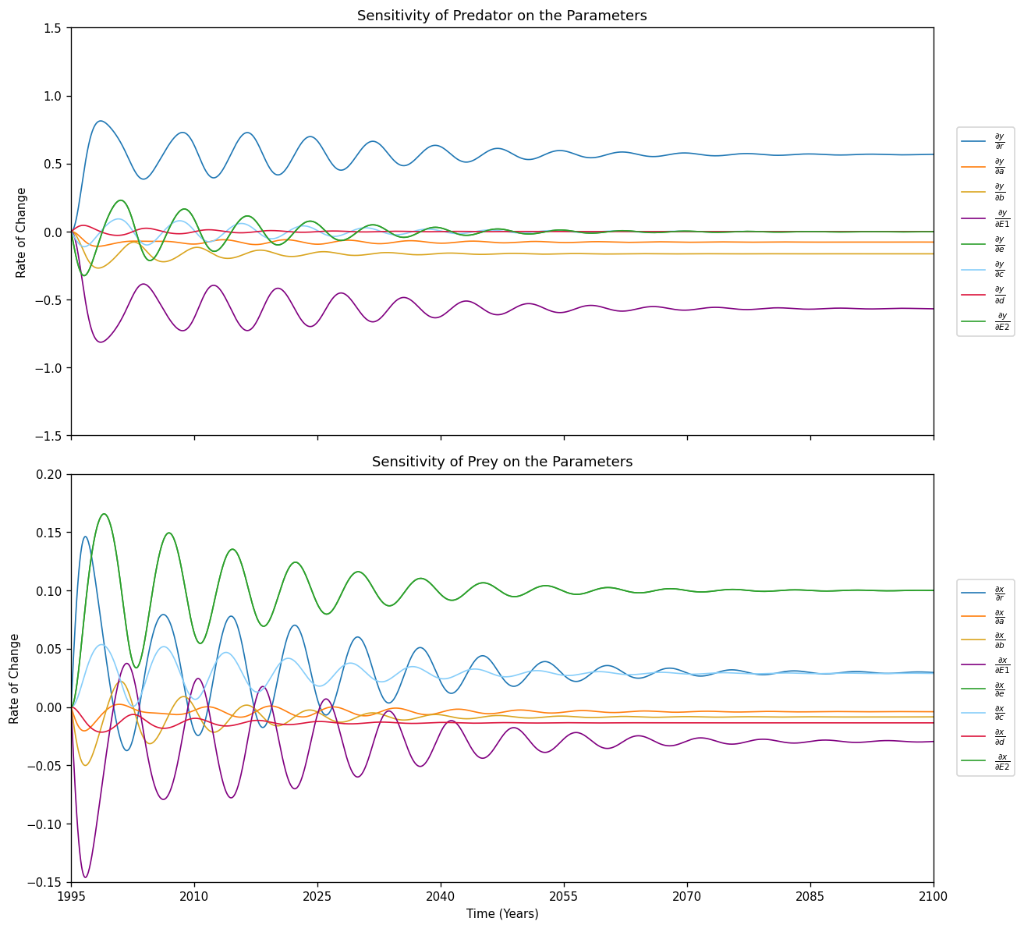
\includegraphics[height=4.6cm, keepaspectratio]{pictures/ch5/fig15_sensitivity.png}\\[2pt]
      {\tiny \textit{Hình 15: Tốc độ thay đổi của Bass \& Menhaden theo 8 tham số}}
    \end{column}
  \end{columns}
\end{frame}

% ------------------------------------------------------------------------------
% SLIDE 24: QUỸ ĐẠO QUẦN THỂ DƯỚI 8 KỊCH BẢN NHIỄU LOẠN THAM SỐ (HÌNH 16)
% ------------------------------------------------------------------------------
\begin{frame}{Quỹ đạo quần thể dưới 8 kịch bản nhiễu loạn tham số (Hình 16)}
  \centering
  \vspace{-0.1cm}
  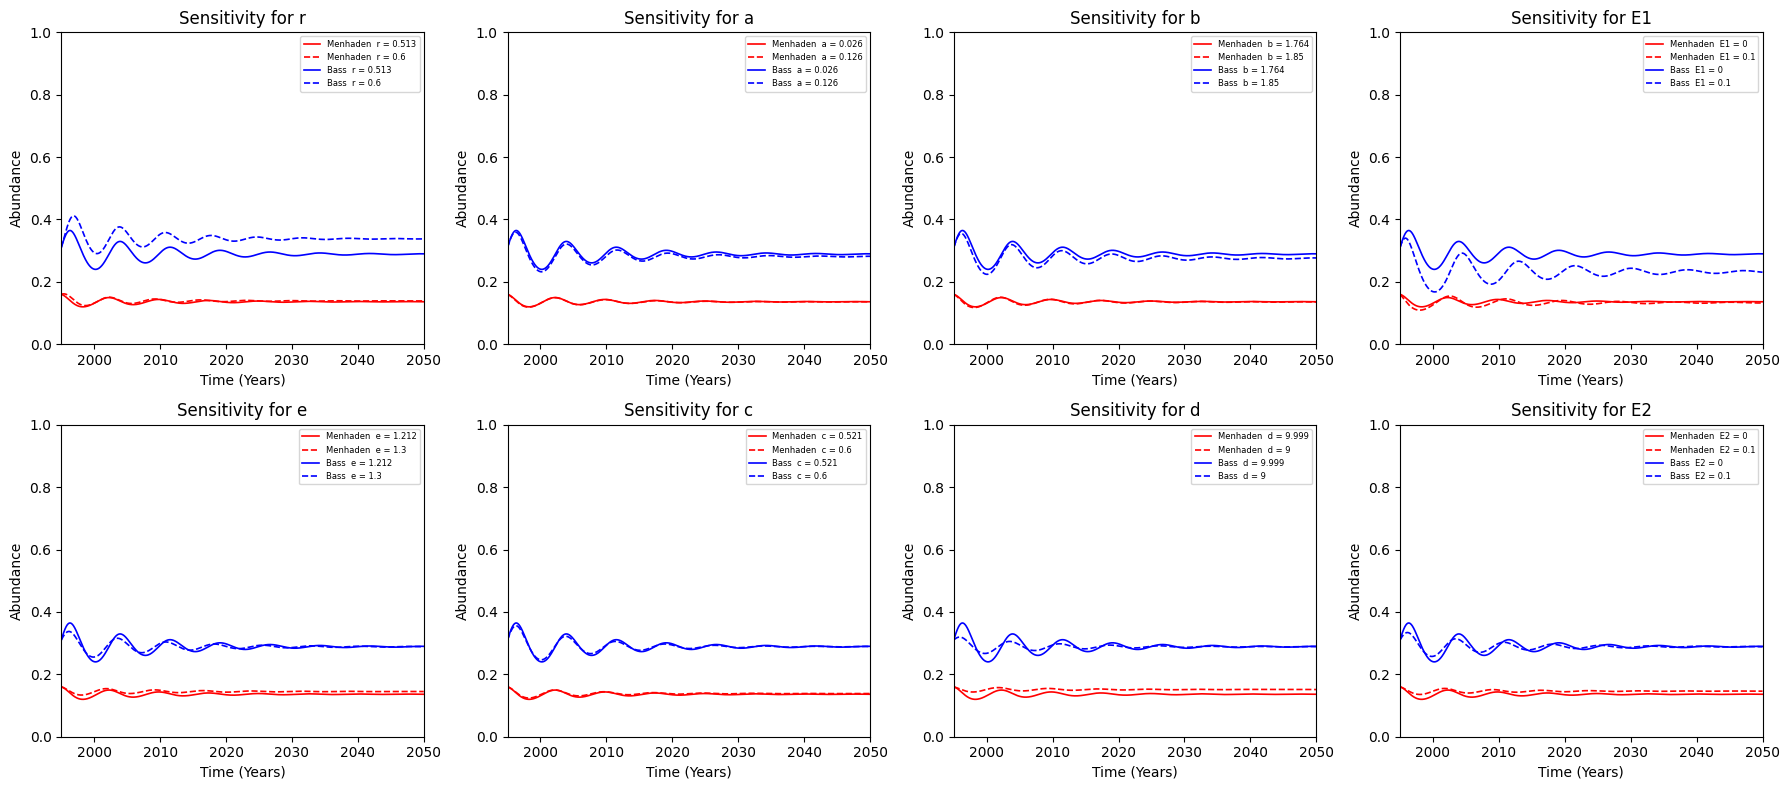
\includegraphics[width=0.98\linewidth, height=0.75\textheight, keepaspectratio]{pictures/ch5/fig16_parameter_perturbations.png}\\[2pt]
  {\scriptsize \textit{Hình 16: Động thái quần thể Menhaden (đỏ) \& Bass (xanh) dưới nhiễu loạn $\pm 10\%$ của 8 tham số ($r, a, b, E_1, e, c, d, E_2$)}}
\end{frame}

% ------------------------------------------------------------------------------
% SLIDE 25: KẾT QUẢ XẾP HẠNG ĐỘ NHẠY TƯƠNG ĐỐI & TÁC ĐỘNG BẤT ĐỐI XỨNG
% ------------------------------------------------------------------------------
\begin{frame}{Xếp hạng độ nhạy tương đối \& Tác động bất đối xứng}
  \begin{columns}[c]
    \begin{column}{0.49\textwidth}
      \begin{block}{\textbf{Độ nhạy chuẩn hóa $\|\bar{S}_{ij}\|_2$}}
        \footnotesize
        \renewcommand{\arraystretch}{1.02}
        \setlength{\tabcolsep}{3pt}
        \begin{tabularx}{\linewidth}{lXlX}
          \toprule
          \multicolumn{2}{c}{\textbf{Menhaden (Mồi)}} & \multicolumn{2}{c}{\textbf{Bass (Săn mồi)}}\\
          \midrule
          $d$ & \textbf{0.9985} & $r$ & \textbf{1.0080}\\
          $e$ & \textbf{0.8886} & $b$ & \textbf{1.0004}\\
          $c$ & $0.1100$        & $e$ & $0.0133$\\
          $b$ & $0.1098$        & $d$ & $0.0093$\\
          $r$ & $0.1079$        & $a$ & $0.0069$\\
          $a$ & $0.0008$        & $c$ & $0.0029$\\
          \midrule
          $E_2$ & \textbf{$0.7328E_2q_2$} & $E_1$ & \textbf{$1.9647E_1q_1$}\\
          $E_1$ & $0.2103E_1q_1$          & $E_2$ & $0.0110E_2q_2$\\
          \bottomrule
        \end{tabularx}\\[3pt]
        \centering{\scriptsize \textit{(Nguồn: Bảng 2 bài báo Panayotova \& Hu, 2023)}}\par
      \end{block}
    \end{column}

    \begin{column}{0.49\textwidth}
      \begin{tcolorbox}[colback=red!5, colframe=red!75!black, arc=1.5mm, left=2.5mm, right=2.5mm, top=1.8mm, bottom=1.8mm]
        \small
        \textbf{Tính chất bất đối xứng sâu sắc:}\\[3pt]
        \footnotesize
        $\blacktriangleright$ Bass nhạy với đánh bắt mòi ($1.965E_1q_1$) gấp \textbf{178 lần} đánh bắt chính bass ($0.011E_2q_2$)!\\
        $\blacktriangleright$ Khai thác quá mức con mồi sẽ tàn phá kẻ săn mồi nhanh hơn nhiều so với đánh bắt trực tiếp.\\
        $\blacktriangleright$ Quản lý đơn loài cá mồi đe dọa trực tiếp cá vược.
      \end{tcolorbox}

      \vspace{0.12cm}
      \begin{block}{\textbf{Hàm ý quản lý sinh thái (EBFM)}}
        \footnotesize
        $\bullet$ \textbf{Nhạy cảm cao:} Tham số nền tảng ($r, b, E_1$ với Bass; $d, e, E_2$ với Menhaden).\\
        $\bullet$ \textbf{Ít nhạy cảm:} Hệ số tương tác cạnh tranh ($a, c$).\\
        $\bullet$ \textbf{Kết luận:} Bắt buộc quản lý tích hợp đa loài, lấy bảo tồn cá mồi làm then chốt.
      \end{block}
    \end{column}
  \end{columns}
\end{frame}

% PHẦN 6: TỔNG KẾT & KHUYẾN NGHỊ QUẢN LÝ (CHƯƠNG 6)
% ==============================================================================
\section{Tổng kết \& Khuyến nghị quản lý (Chương 6)}



% ------------------------------------------------------------------------------
% SLIDE 25: TỔNG KẾT KẾT QUẢ ĐẠT ĐƯỢC (CHƯƠNG 6)
% ------------------------------------------------------------------------------
\begin{frame}{Tổng kết các kết quả chính đạt được của đề tài (Chương 6)}
  \begin{columns}[t]
    \begin{column}{0.49\textwidth}
      \begin{block}{\textbf{1. Đặt đúng mô hình toán học}}
        \footnotesize
        \begin{itemize}
          \item Chứng minh nghiệm $x(t) \ge 0, y(t) \ge 0$ và bị chặn toàn cục trong tập bất biến sinh học:
          $$\Omega = \left\{ (x, y) \in \mathbb{R}^2_+ \;\middle|\; x \le \frac{r}{a}, \; x + \frac{y}{\gamma} \le L \right\}$$
          \item Bảo đảm tính hợp lý và đúng đắn sinh học.
        \end{itemize}
      \end{block}

      \vspace{0.1cm}

      \begin{block}{\textbf{2. Khớp mô hình \& Dự báo}}
        \footnotesize
        \begin{itemize}
          \item Tái hiện chuẩn xác chuỗi dữ liệu 23 năm ($S = 0.11$).
          \item Điểm dừng $Q = (0.1363, 0.2886)$ ổn định tiệm cận; chu kỳ hồi phục 13 năm.
        \end{itemize}
      \end{block}
    \end{column}

    \begin{column}{0.49\textwidth}
      \begin{block}{\textbf{3. Luận cứ bác bỏ MSY đơn loài}}
        \footnotesize
        \begin{itemize}
          \item Chỉ ra sự phi lý khi áp dụng MSY độc lập cho cá mồi.
          \item Chứng minh sự cần thiết phải \textbf{cắt giảm 50\% hạn ngạch đánh bắt cá mòi dầu} để bảo tồn chuỗi thức ăn.
        \end{itemize}
      \end{block}

      \vspace{0.1cm}

      \begin{exampleblock}{\textbf{4. Phân tích độ nhạy cục bộ (DDM)}}
        \footnotesize
        \begin{itemize}
          \item Xếp hạng các mắt xích chi phối mạnh nhất:
          \begin{itemize}
            \item Cá vược nhạy nhất với $r$ ($\|S\| \approx 1.008$), $b$ ($\approx 1.000$) và nỗ lực $E_1$.
            \item Định hướng cơ quan quản lý kiểm soát đúng trọng tâm.
          \end{itemize}
        \end{itemize}
      \end{exampleblock}
    \end{column}
  \end{columns}
\end{frame}

% ------------------------------------------------------------------------------
% SLIDE 26: HÀM Ý CHÍNH SÁCH QUẢN LÝ CHO VỊNH CHESAPEAKE (CHƯƠNG 6)
% ------------------------------------------------------------------------------
\begin{frame}{Hàm ý chính sách quản lý cho Vịnh Chesapeake (Chương 6)}
  \begin{columns}[t]
    \begin{column}{0.32\textwidth}
      \begin{block}{\centering \textbf{Chuyển dịch sang EBFM}}
        \scriptsize
        \begin{itemize}
          \item Bỏ hẳn tư duy quản lý đơn loài truyền thống đối với các loài cá mồi ven biển.
          \item Tích hợp đầy đủ nhu cầu dinh dưỡng đa loài vào các chỉ tiêu quản lý nghề cá Đại Tây Dương (ASMFC).
        \end{itemize}
      \end{block}
    \end{column}

    \begin{column}{0.32\textwidth}
      \begin{block}{\centering \textbf{Thiết lập chỉ số ERP}}
        \scriptsize
        \begin{itemize}
          \item Ban hành \textbf{Điểm tham chiếu sinh thái} (\textit{ERP}) nghiêm ngặt đối với cá mòi dầu.
          \item Giữ lại ít nhất \textbf{50\%} sinh khối cá mòi dầu trong nước làm thức ăn cho cá vược sọc và chim biển.
        \end{itemize}
      \end{block}
    \end{column}

    \begin{column}{0.32\textwidth}
      \begin{block}{\centering \textbf{Kiểm soát tàu công nghiệp}}
        \scriptsize
        \begin{itemize}
          \item Siết chặt hạn ngạch đánh bắt (\textit{harvest caps}) của các tập đoàn tàu vây công nghiệp (như Omega Protein).
          \item Bảo vệ các bãi đẻ nước ngọt và vùng nước lợ sinh sản của cá vược sọc.
        \end{itemize}
      \end{block}
    \end{column}
  \end{columns}

  \vspace{0.25cm}
  \begin{alertblock}{\centering \textbf{Nguyên tắc cốt lõi:}}
    \centering \footnotesize \textit{Bảo vệ cá mòi dầu chính là bảo vệ nguồn sinh kế hàng tỷ USD từ nghề cá thương mại và du lịch câu cá giải trí của cá vược sọc!}
  \end{alertblock}
\end{frame}

% ------------------------------------------------------------------------------
% SLIDE 27: HẠN CHẾ & HƯỚNG PHÁT TRIỂN TIẾP THEO (CHƯƠNG 6)
% ------------------------------------------------------------------------------
\begin{frame}{Đánh giá hạn chế \& Hướng phát triển tiếp theo (Chương 6)}
  \begin{columns}[t]
    \begin{column}{0.49\textwidth}
      \begin{alertblock}{\textbf{Hạn chế của mô hình hiện tại}}
        \footnotesize
        \begin{itemize}
          \item \textbf{Bỏ qua cấu trúc tuổi:} Mô hình chưa phân biệt cá con, cá trưởng thành và cá sinh sản (\textit{age-structured}).
          \item \textbf{Giới hạn ở hệ 2 loài:} Chưa xét cạnh tranh trực tiếp với các loài săn mồi khác như cá xanh (\textit{Bluefish}), cá yếu, cá mập cát.
          \item \textbf{Mô hình xác định thuần túy:} Chưa tính các yếu tố nhiễu loạn ngẫu nhiên từ môi trường (nhiệt độ mùa đông, bão lũ, ô nhiễm đột xuất).
        \end{itemize}
      \end{alertblock}
    \end{column}

    \begin{column}{0.49\textwidth}
      \begin{exampleblock}{\textbf{Định hướng nghiên cứu mở rộng}}
        \footnotesize
        \begin{itemize}
          \item \textbf{Mô hình hóa phân lớp tuổi:} Xây dựng hệ phương trình vi phân có độ trễ (\textit{DDE}) hoặc ma trận Leslie kết hợp kích thước mắt lưới đánh bắt.
          \item \textbf{Mạng lưới thức ăn đa loài:} Mở rộng lên hệ 4--5 loài (Menhaden -- Striped Bass -- Bluefish -- Chim ưng biển).
          \item \textbf{Tích hợp ngẫu nhiên \& Khí hậu:} Ứng dụng hệ phương trình vi phân ngẫu nhiên (\textit{SDEs}) khảo sát tác động của biến đổi khí hậu toàn cầu.
        \end{itemize}
      \end{exampleblock}
    \end{column}
  \end{columns}
\end{frame}

% ------------------------------------------------------------------------------
% SLIDE 28: KẾT LUẬN & HỎI ĐÁP (Q&A)
% ------------------------------------------------------------------------------
\begin{frame}[plain]
  \begin{tikzpicture}[remember picture, overlay]
    \fill[OceanNavy] (current page.north west) rectangle ($(current page.north east) + (0, -2.4cm)$);
    \fill[OceanTeal] ($(current page.north west) + (0, -2.4cm)$) rectangle ($(current page.north east) + (0, -2.55cm)$);
    \fill[OceanNavy] (current page.south west) rectangle ($(current page.south east) + (0, 0.7cm)$);
  \end{tikzpicture}

  \vspace*{-0.4cm}
  \begin{columns}[c]
    \begin{column}{0.18\textwidth}
      \centering
      \IfFileExists{logo_hus.png}{%
        
\includegraphics[height=1.8cm, keepaspectratio]{logo_hus.png}
      }{%
        \begin{tikzpicture}
          \draw[thick, white, fill=OceanBlue!60] (0,0) circle (0.9cm);
          \node[white, font=\scriptsize\bfseries, align=center] at (0,0) {HUS\\VNU};
        \end{tikzpicture}
      }
    \end{column}
    \begin{column}{0.80\textwidth}
      {\color{white}\small \textbf{KHOA TOÁN -- CƠ -- TIN HỌC $\bullet$ ĐH KHOA HỌC TỰ NHIÊN}}\\[2pt]
      {\color{white}\large \textbf{BÁO CÁO TIỂU LUẬN: CÁC MÔ HÌNH TOÁN ỨNG DỤNG}}
    \end{column}
  \end{columns}

  \vspace{0.8cm}

  \begin{center}
    {\Huge \color{OceanNavy} \textbf{XIN CHÂN THÀNH CẢM ƠN!}}\\[0.3cm]
    {\large \color{OceanBlue} \textbf{THẦY CÔ VÀ CÁC BẠN ĐÃ LẮNG NGHE BÀI THUYẾT TRÌNH}}\\[0.6cm]

    \begin{tcolorbox}[colback=OceanLight, colframe=OceanNavy, arc=2mm, width=0.65\textwidth]
      \centering
      {\large \color{OceanNavy} \textbf{PHIÊN THẢO LUẬN \& HỎI ĐÁP (Q\&A)}}\\[0.2cm]
      {\footnotesize Nhóm sinh viên rất mong nhận được những góp ý quý báu từ TS. Nguyễn Trọng Hiếu và các bạn sinh viên!}
    \end{tcolorbox}
  \end{center}
\end{frame}

\end{document}
